\documentclass[handout]{beamer}
\usepackage{graphicx}
\usepackage{caption}
\usepackage{subcaption}
\usepackage{tikz}
\usepackage{wrapfig}
\graphicspath{ {../thesis/img/}{./img} }
\usetheme{default}

\title{Molecular dynamics study of ideal polymer chains with variable persistence length}
\subtitle{Bachelor thesis defense}
\author{Yahor Paromau}
\institute{ITP@IPF}
\date{12.12.2023}

\newcommand{\mean}[1]{\langle #1 \rangle}
\newcommand{\E}[1]{\langle#1\rangle}

\begin{document}


\begin{frame}
    \titlepage
\end{frame}


\begin{frame}
    \frametitle{Outline}
    \tableofcontents
\end{frame}

\section{Introduction and Motivation}

% Motivation - context ---------------------------------------------------------------------------

\begin{frame}
    \frametitle{Motivation - context}
    \begin{center}
        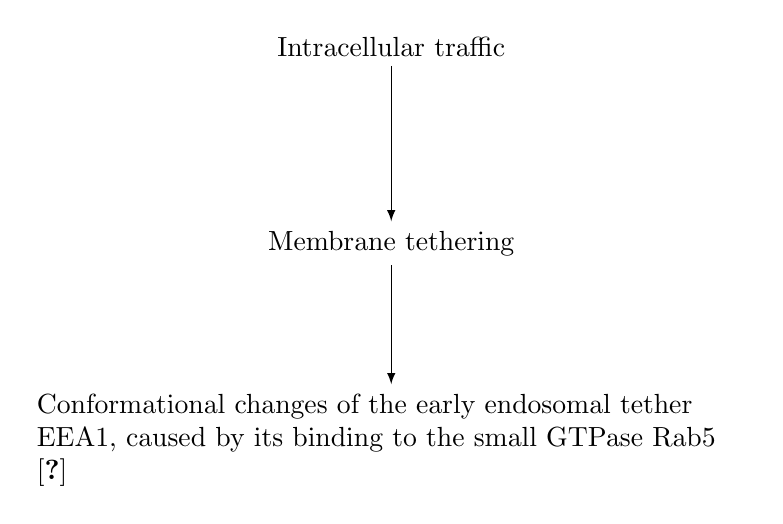
\begin{tikzpicture}[>=latex, node distance=2.5cm]
        
        \node (intracellular) {Intracellular traffic};
        \node (tethering) [below of=intracellular] {Membrane tethering};
        \node (conformational) [below of=tethering,text width=9cm] {
            Conformational changes of the early endosomal tether EEA1,
            caused by its binding to the small GTPase Rab5
            \cite{Murray2016}
            };
        
        \draw[->] (intracellular) -- (tethering);
        \draw[->] (tethering) -- (conformational);
        
        \end{tikzpicture}
    \end{center}
\end{frame}

% Motivation - Quantities ---------------------------------------------------------------------------

\begin{frame}
    \frametitle{Quantities - MSD and scaling exponent}
    \begin{itemize}
        \item Mean squared displacement (MSD) of the chain end (MSDLM):
        $$\E{[\Delta\vec{r}_N(t)]^2} := \E{[\vec{r}_N(t)-\vec{r}_N(0)]^2}$$
        \item (Local) scaling exponent alpha of the MSD \cite{Singh:2022}
        $$\E{[\Delta\vec{r}_N(t)]^2} \propto t^{\alpha(t)}$$
    \end{itemize}
\end{frame}

% Motivation - paper ---------------------------------------------------------------------------

\begin{frame}
    \frametitle{Motivation - experimental study}
    \begin{figure}[h]
        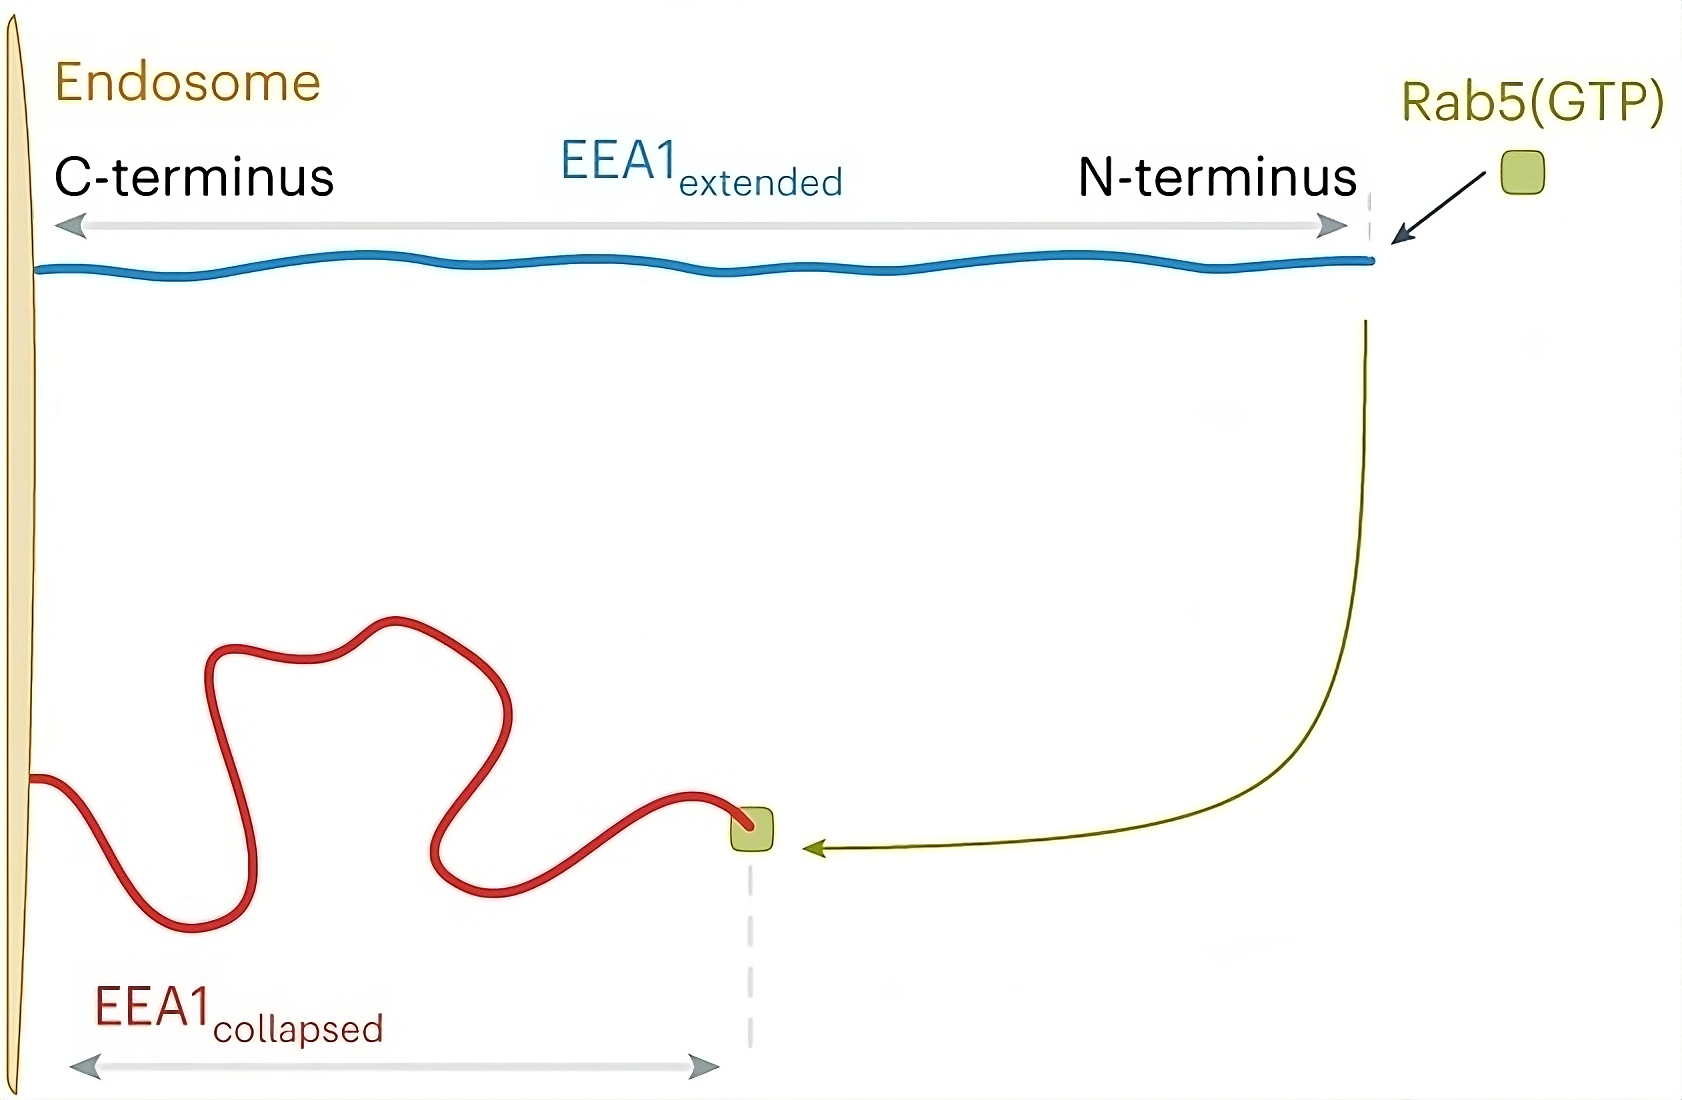
\includegraphics[height=6.9cm]{./Singh_intro_a.png}
        \caption{
            Sketch of extended/collapsed states of EEA1 upon the binding of Rab5
            \cite{Singh:2022}
        }
    \end{figure}
\end{frame}

% Motivation - paper ---------------------------------------------------------------------------

\begin{frame}
    \frametitle{Motivation - experimental study}
    \framesubtitle{MSD and local scaling exponent}
    \centering
    \begin{figure}[h]
        \centering
        \begin{subfigure}[b]{0.49\textwidth}
            \centering
            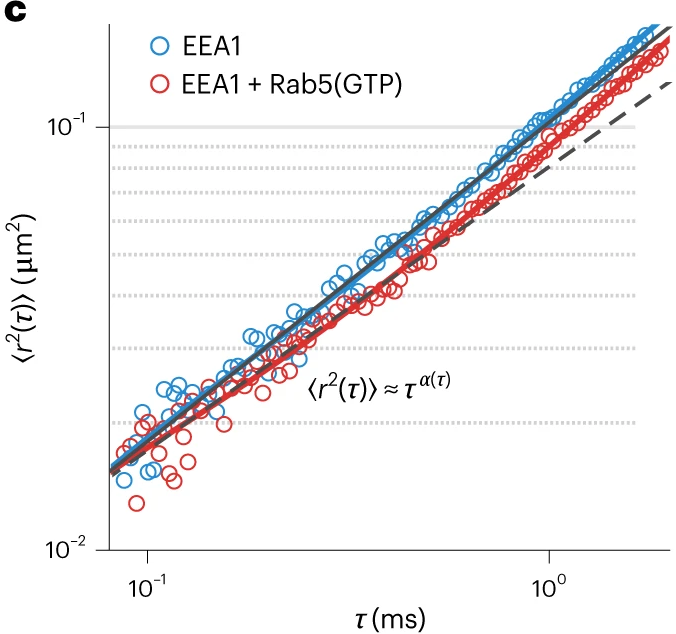
\includegraphics[width=\textwidth]{./Singh_intro_с.png}
        \end{subfigure}
        \begin{subfigure}[b]{0.49\textwidth}
            \centering
            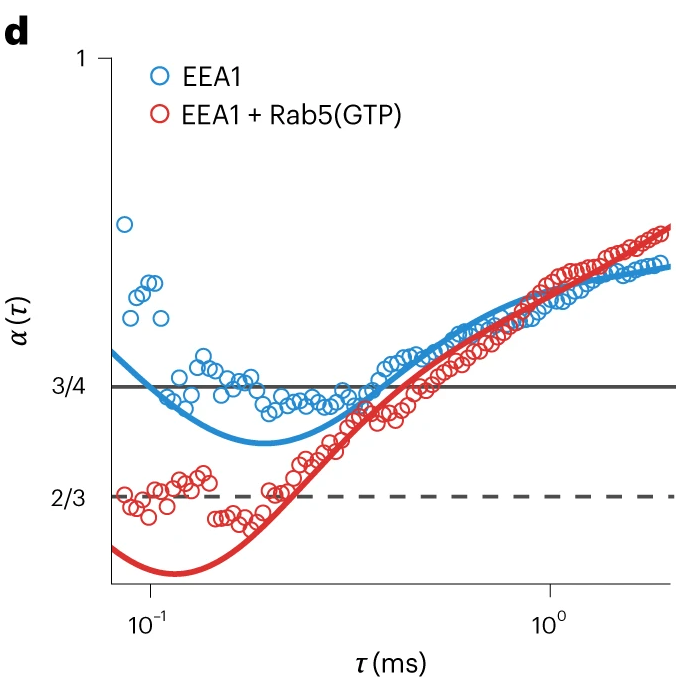
\includegraphics[width=\textwidth]{./Singh_intro_d.png}
        \end{subfigure}
        \caption{
            \textbf{c)} Mean square displacement (MSD) and \textbf{d)}
            local scaling exponent $\alpha$ of the MSD \cite{Singh:2022}
        }
    \end{figure}

\end{frame}

% Motivation - summary ---------------------------------------------------------------------------

\begin{frame}
    \frametitle{Motivation - summary}
    \begin{itemize}
        \item Change of stiffness is shown indirectly by fitting the 
        analytical expression to the experimentally observed data before/after
        the binding $\Rightarrow$ might be other impact factors (complex system)
        \item Free chains are measured, however by the membrane tethering the EEA1 
        chain is anchored to the endosome
        \item The dynamics of anchored semiflexible chains is not yet well studied 
    \end{itemize} 
\end{frame}

% Goals ---------------------------------------------------------------------------

\begin{frame}
    \frametitle{Motivation/Goals}

    Using the molecular dynamics:
    \vspace{0.5cm}
    \begin{itemize}
        \item Study dynamical properties of the anchored
        semiflexible chains by varying stiffness and friction of the chain end
        \item Change in mechanical properties (chain stiffness, friction coefficient of the chain end)
        "$\Rightarrow$" change in scaling behavior of the MSD as in \cite{Singh:2022}? 
    \end{itemize}

\end{frame}

\begin{frame}
    \frametitle{Limitations}

    \begin{itemize}
        \item No hydrodynamic interactions
        \item Ideal chains
    \end{itemize}

\end{frame}

\section{Anchored chain dynamics}

\subsection{Comparison to free chain}

\begin{frame}
    \frametitle{Anchored fully flexible chains}
    \framesubtitle{MSD: $\mean{[\Delta R(t)]^2}$ - free vs anchored chains}

    \begin{figure}[h]
        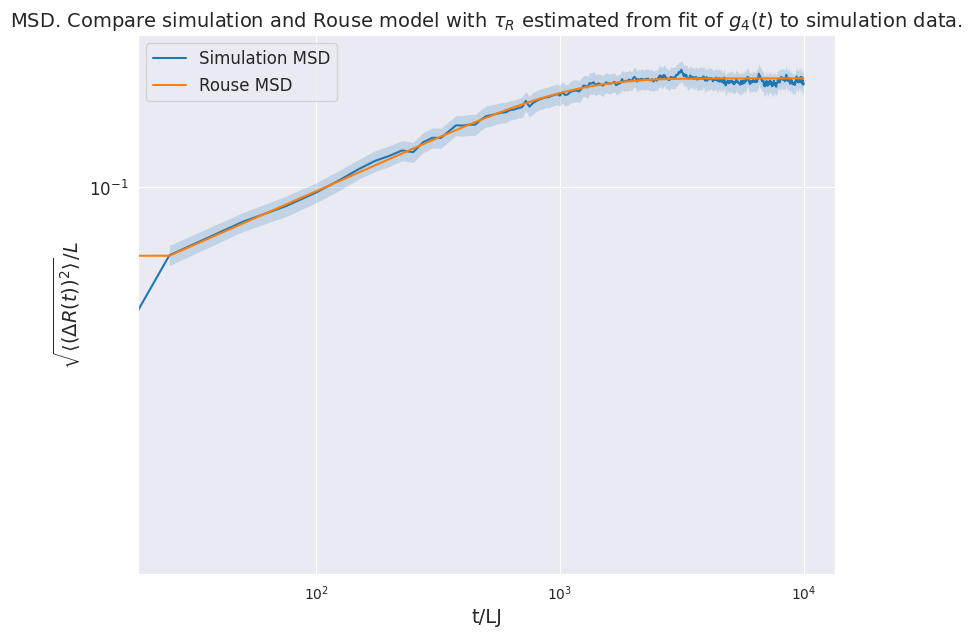
\includegraphics[trim={0.1cm 0.1cm 0.1cm 1cm},clip,width=\textwidth]{./3-exp-free-param-log.png}
        \caption{
            MSD - compare simulation of free chains, anchored chains and Rouse model,
            $\frac{\tau_{R, \textrm{empirical,anchored}}}{\tau_{R, \textrm{analytical, free}}} \approx 4.47$
        }
        \label{fig:full-flex-chain-free-log}
    \end{figure}
\end{frame}

\subsection{Impact of chain stiffness}

% Semiflexible anchored - Equations -------------------------------------------------------------------

\begin{frame}
    \frametitle{Anchored semiflexible chains - impact of stiffness}
    \framesubtitle{Used equations}

    Kuhn length \cite{svaneborg_2020}:
    \begin{equation}
        l_K = l_b \frac{2\kappa + e^{-2 \kappa} - 1}{1-e^{-2\kappa}(2 \kappa + 1)}
    \end{equation}
    Number of Kuhn segments:
    \begin{equation} 
        N_K = \frac{L}{l_K}
    \end{equation}
    Rouse time:
    \begin{equation} \label{eq:tau_R_kuhn}
        \tau_R = \frac{1}{3 \pi^2} \frac{\zeta_{K} \mean{R^2}}{k_B T} = \frac{1}{3 \pi^2} \frac{\zeta N_b N_K l_K^2}{k_B T}
    \end{equation}
\end{frame}

% Semiflexible anchored - MSD ---------------------------------------------------------------------------

\begin{frame}
    \frametitle{Anchored semiflexible chains - impact of stiffness}
    \framesubtitle{MSD: $\mean{[\Delta R(t)]^2}$}

    \begin{figure}
        \centering
        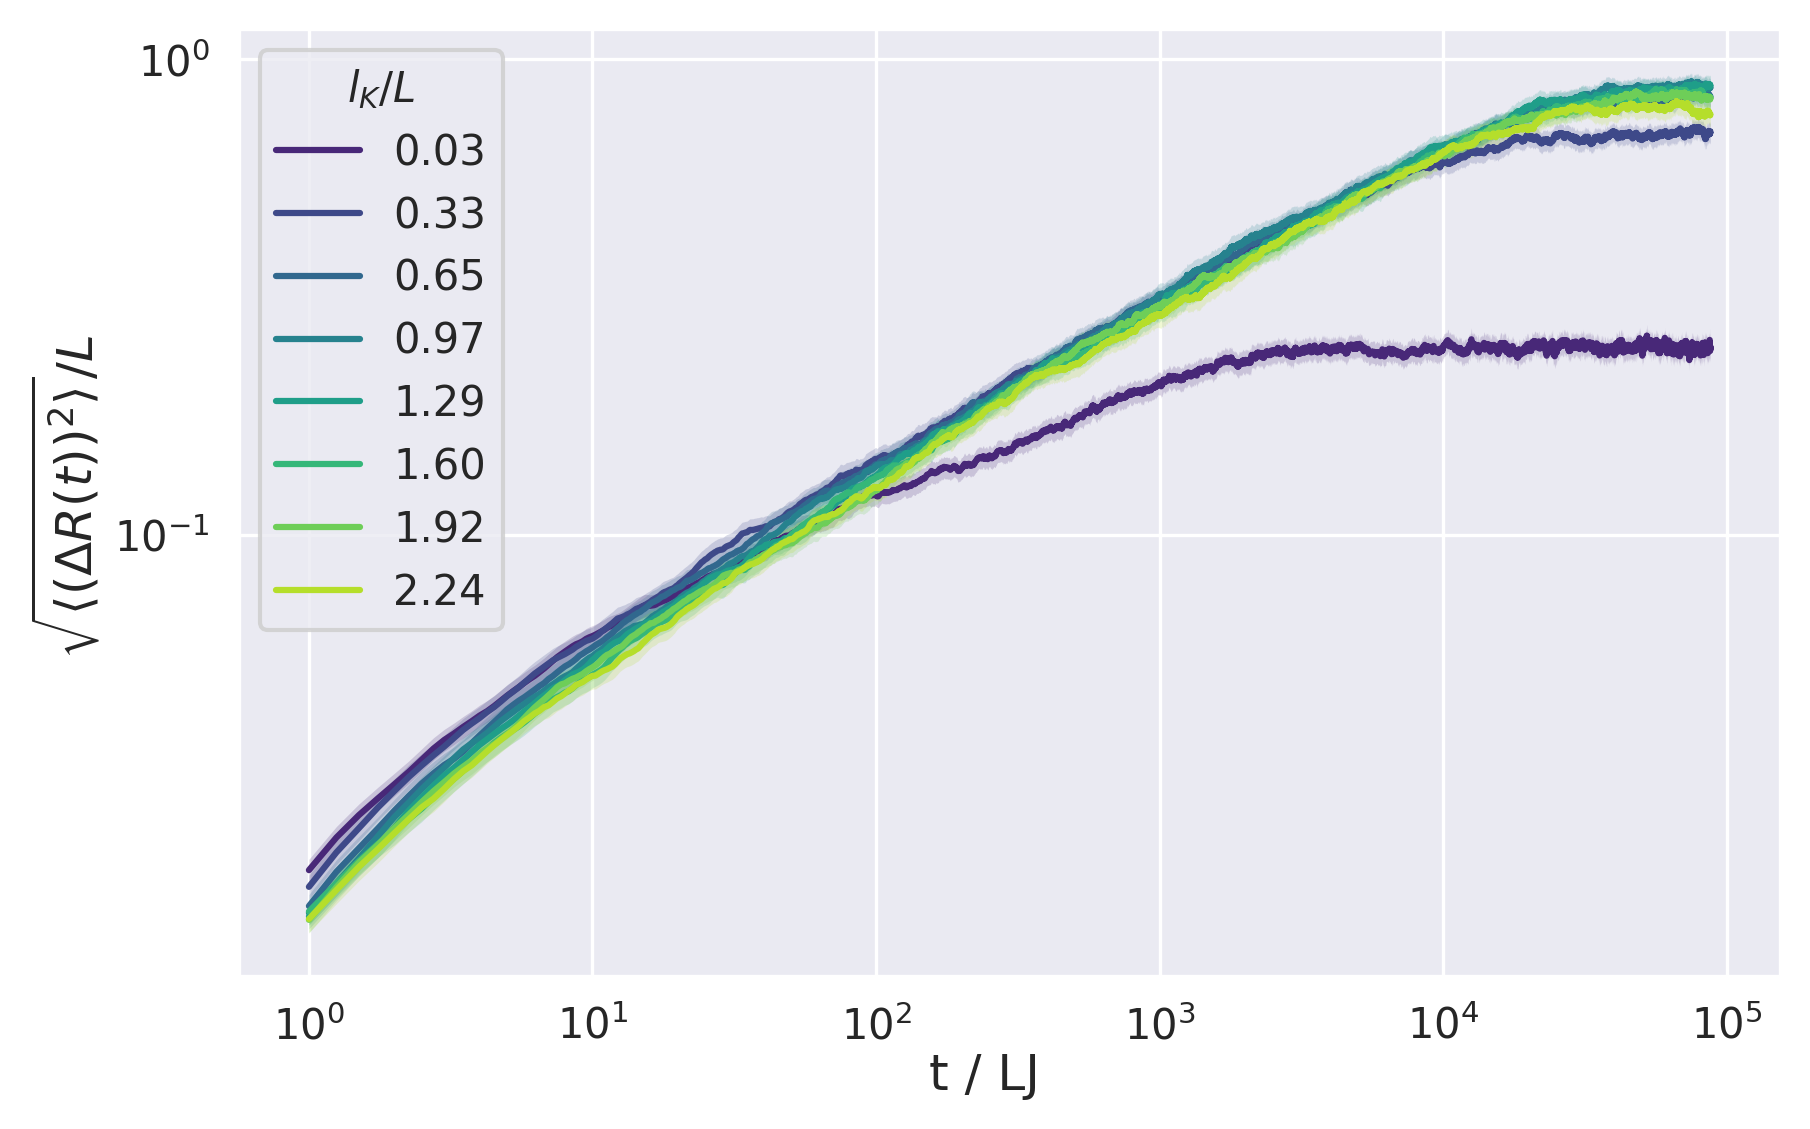
\includegraphics[width=\columnwidth,trim={0cm 0cm 0cm 0.0cm},clip]{4-exp-delta_R-bare-log.png}
        \caption{Empirical MSD of ETE of anchored chains with different Kuhn length values.}
        \label{fig:msd_anchored_l_K}
    \end{figure}
\end{frame}

% Semiflexible anchored - MSD vs Adjusted Rouse ---------------------------------------------------------------------------

\begin{frame}
    \frametitle{Anchored semiflexible chains - impact of stiffness}
    \framesubtitle{MSD $\mean{[\Delta R(t)]^2}$ vs Adjusted Rouse with $\tau_R$, $a$ as free parameters}
    $$ \mean{[\Delta R(t)]^2} = a \mean{R} [1 - \exp(-\frac{t}{\tau_R})] $$
    \begin{figure}[h]
        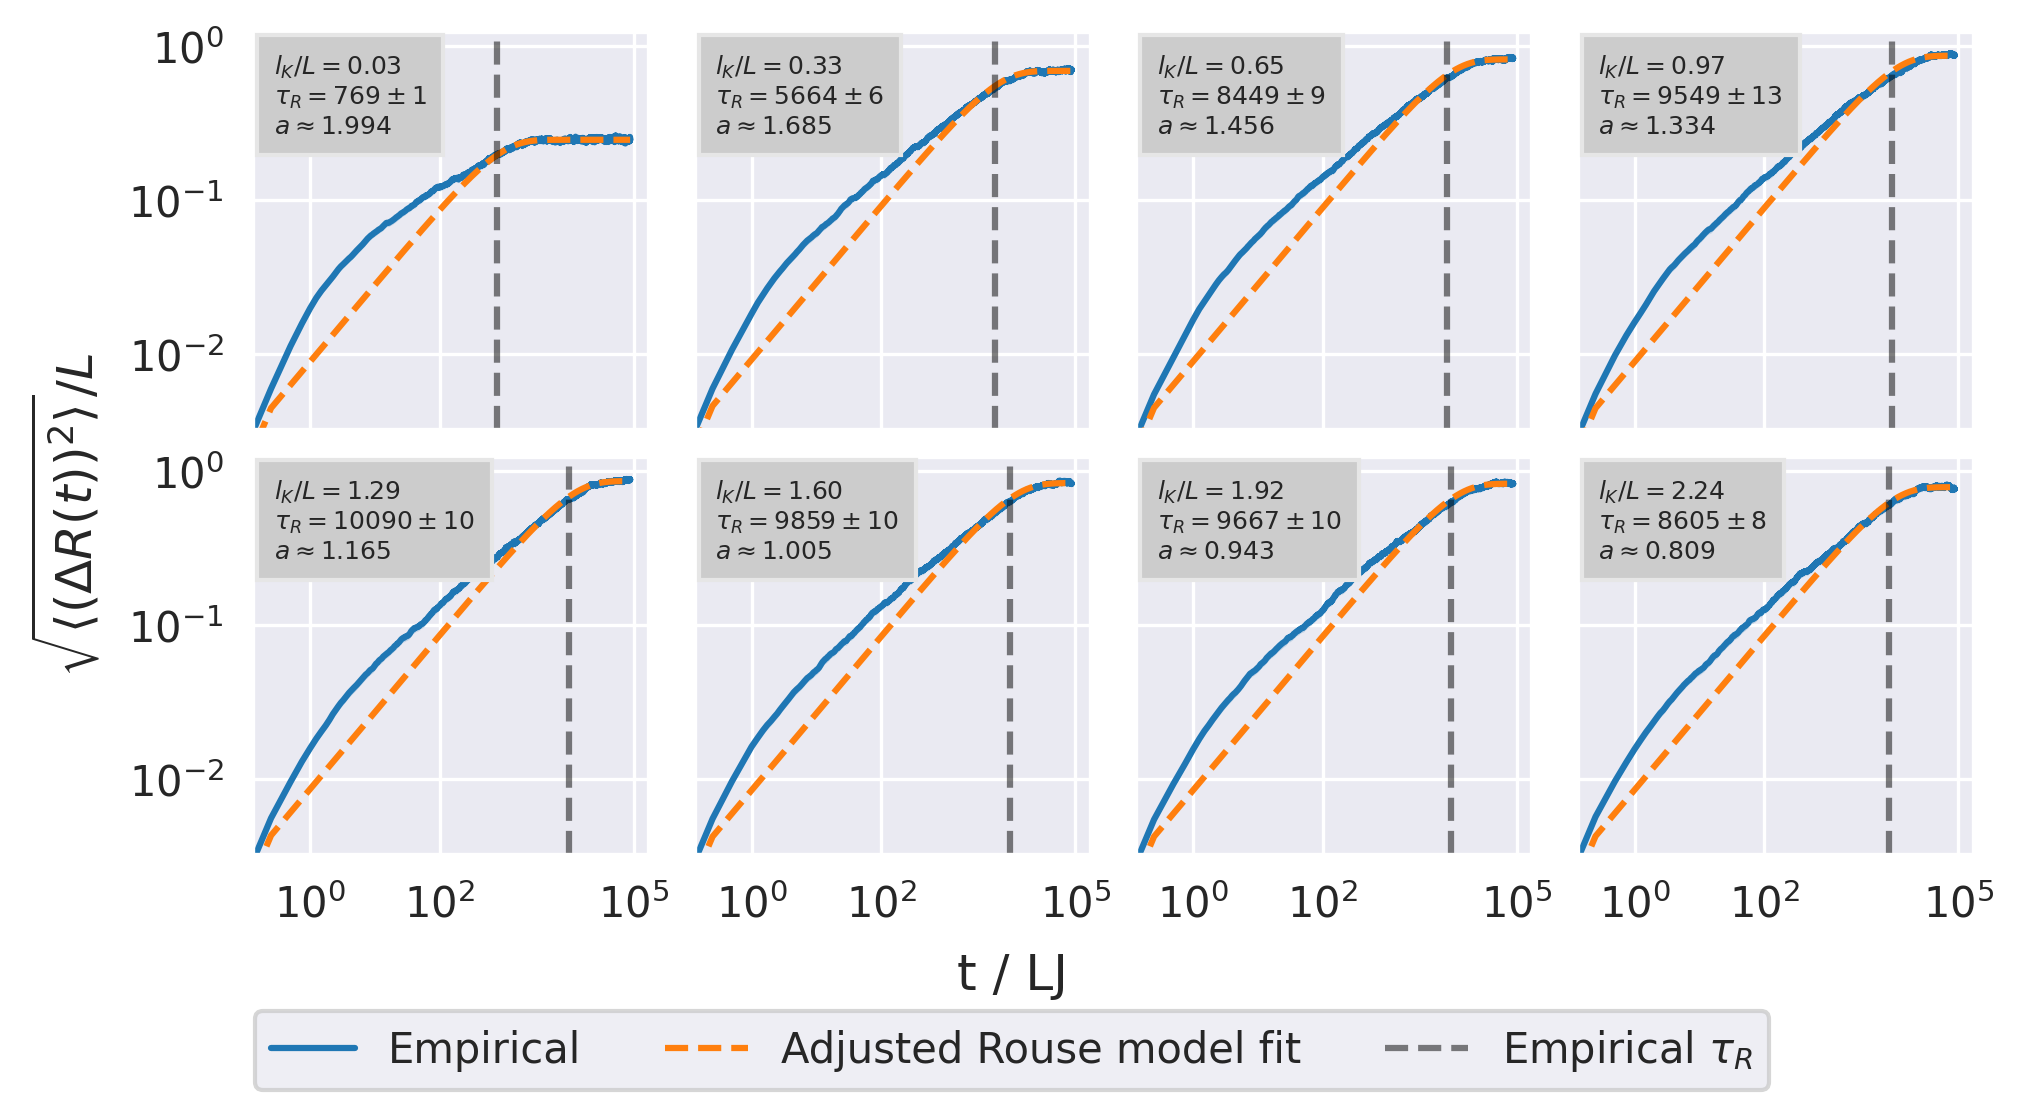
\includegraphics[width=11cm]{4-exp-delta_R-rouse_fit-tau-a_log.png}
    \end{figure}
\end{frame}

% Semiflexible anchored - alpha ---------------------------------------------------------------------------

\begin{frame}
    \frametitle{Anchored semiflexible chains - impact of stiffness}
    \framesubtitle{Scaling behavior}
    \begin{figure}[h]
        \begin{center}
          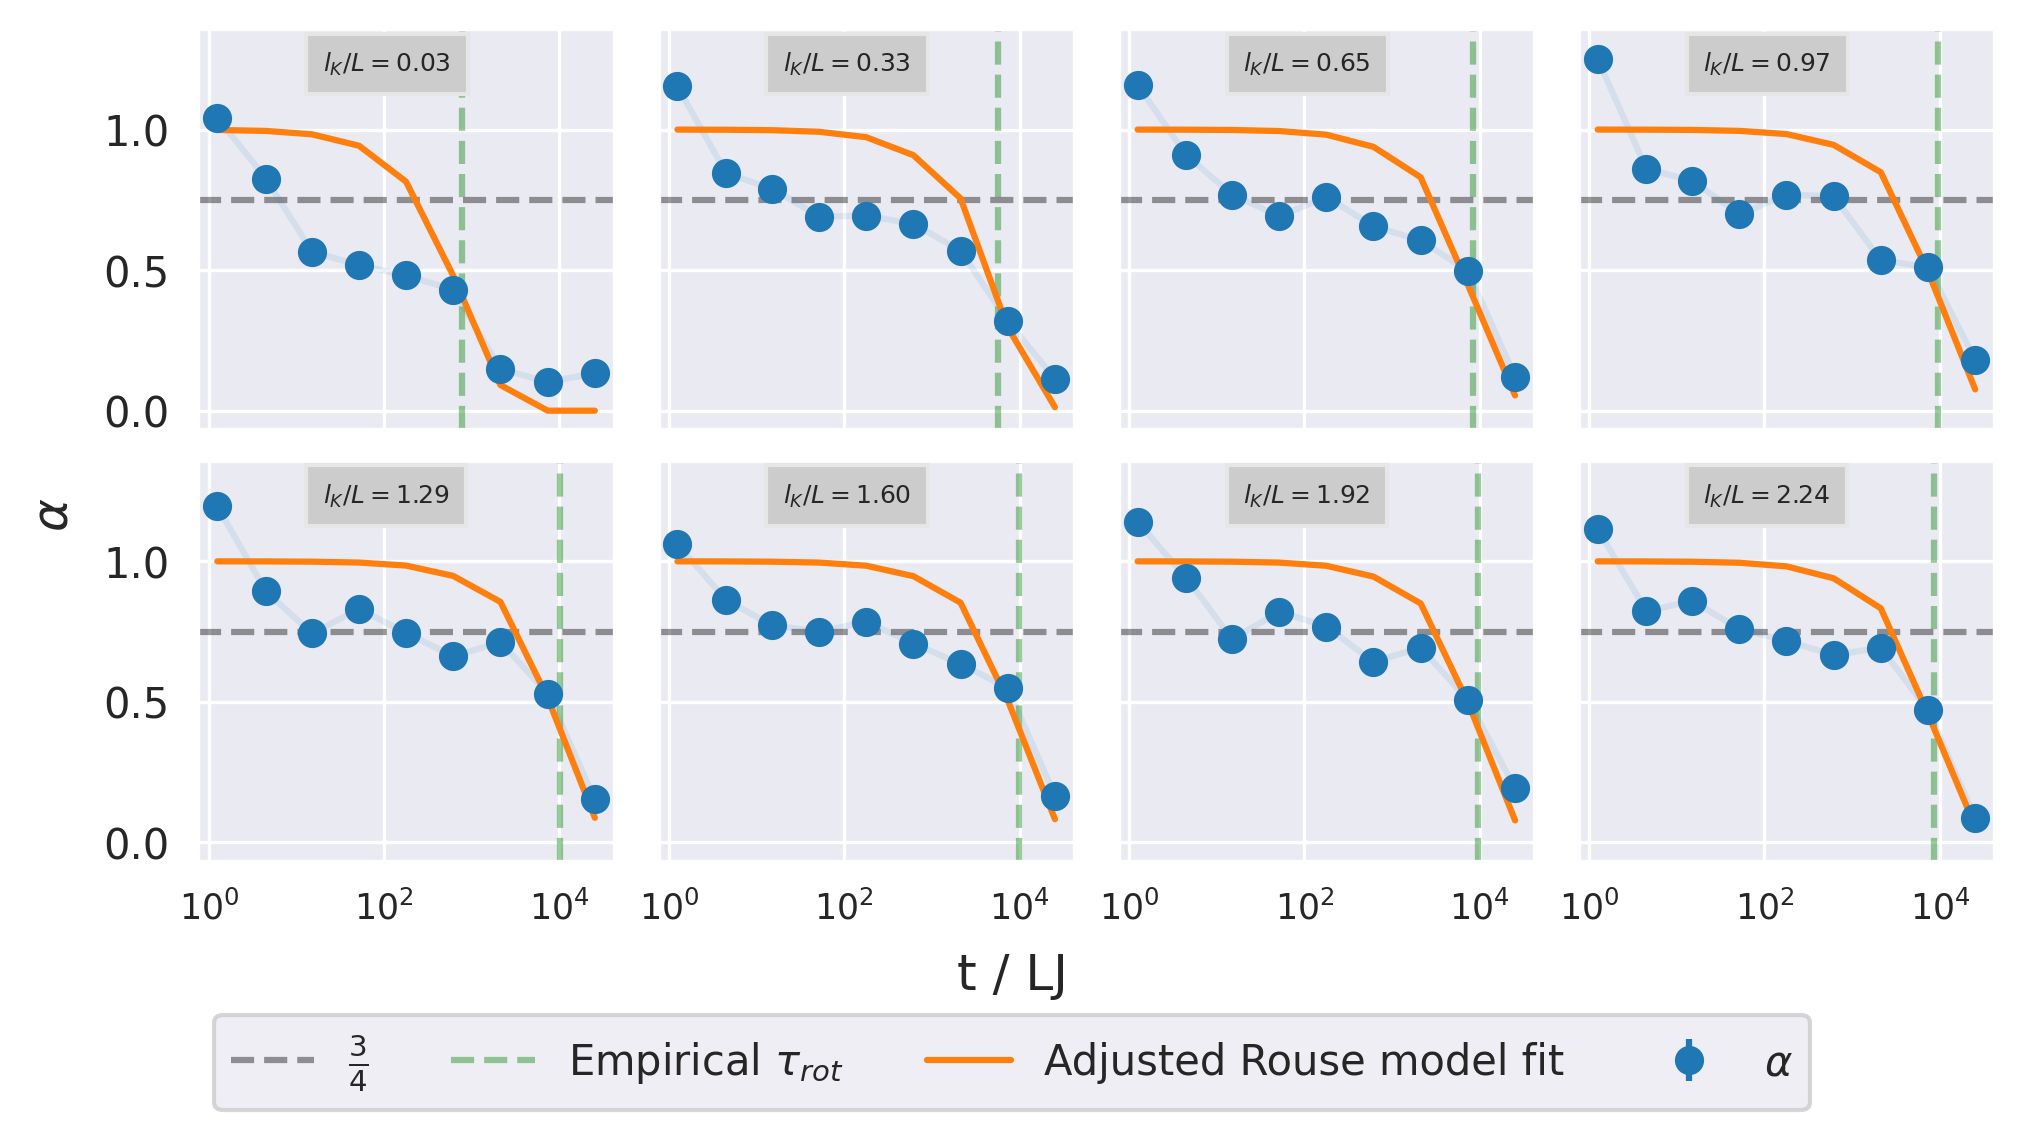
\includegraphics[width=\columnwidth,trim={0cm 0cm 0cm 0.0cm},clip]{4-exp-delta_R-rouse_fit-tau-a_alpha.png}
          \caption{\label{fig:alpha_anchored_l_K}
          Scaling exponent $\alpha$ of the MSD of ETE of anchored semiflexible chain (blue points) and 
          scaling exponent $\alpha$ of the Adjusted Rouse model prediction for semi-flexible chains 
          (orange line).
          }
        \end{center}
    \end{figure}
\end{frame}

% Semiflexible anchored - by dim ---------------------------------------------------------------------------

\begin{frame}
    \frametitle{Anchored semiflexible chains - impact of stiffness}
    \framesubtitle{Separation of the dynamics into components parallel and perpendicular to the main-axis}

    \begin{figure}[h]
        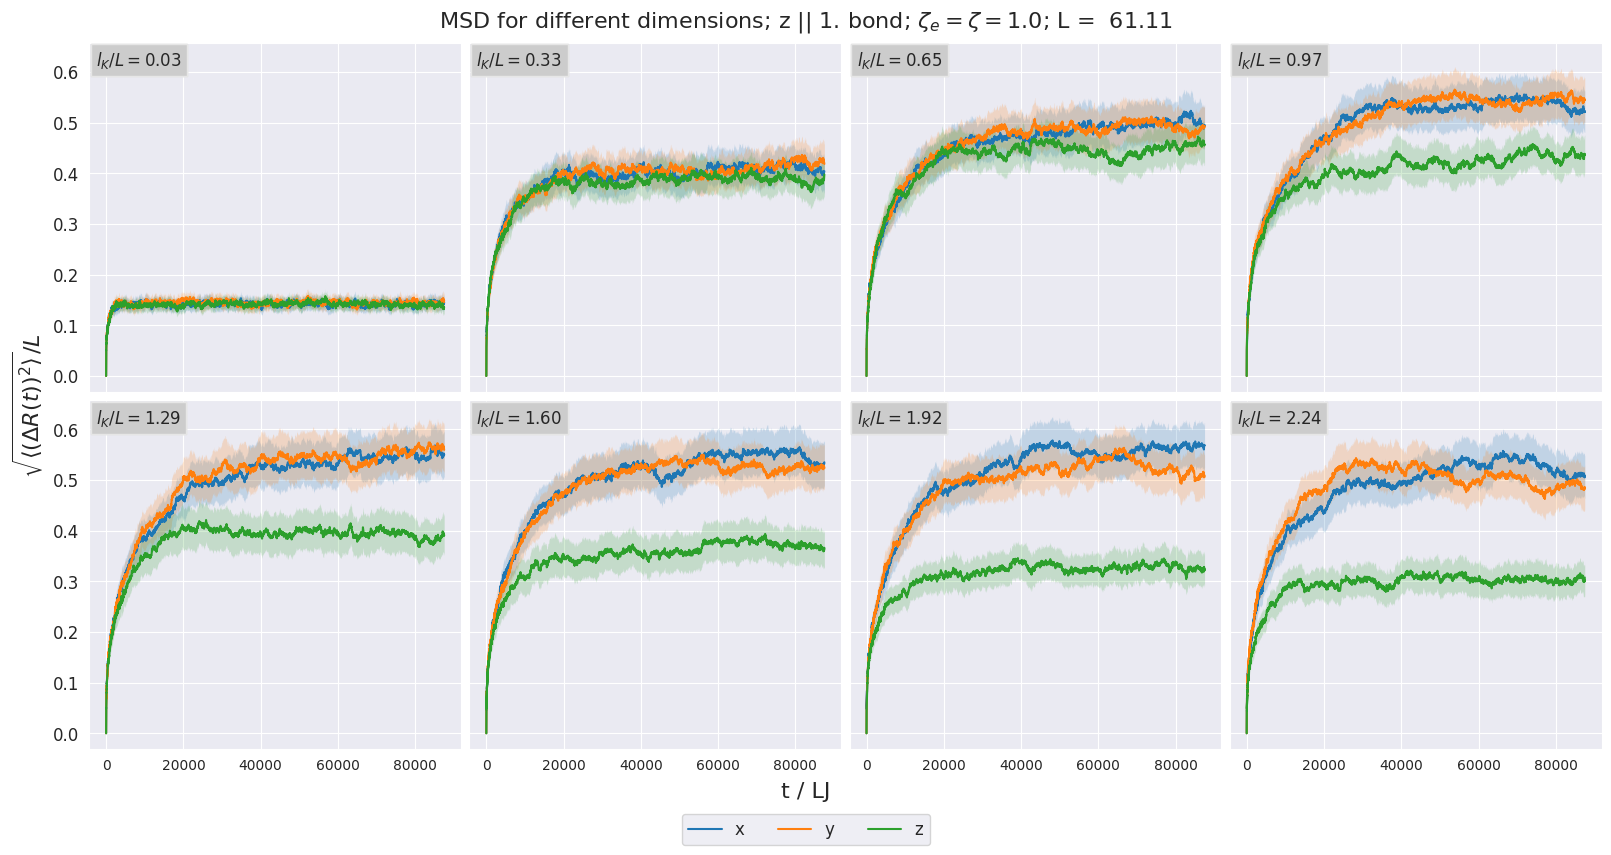
\includegraphics[width=11cm]{./4-exp-msd_by_dim.png}
        \caption{
            Empirical MSD of ETE of anchored chains with different Kuhn length values,
            separated in components parallel and perpendicular to the main-axis
        }
    \end{figure}
\end{frame}

% Semiflexible anchored impact of stifness - conclusions --------------------------------

\begin{frame}
    \frametitle{Anchored semiflexible chains - impact of stiffness}
    \framesubtitle{Conclusions}

    \begin{enumerate}
        \item The behavior of MSD for different $l_K$ is roughly the same for $l_K/L \gtrapprox 0.65$
        \item The relaxation time grows non-linearly with rising $l_K$
        \item MSD in z dimension is noticable different for $l_K \gtrapprox 0.97$. 
        \begin{itemize}
            \item The relaxation time in z dimension gets smaller 
            relative to x,y dimensions with increasing $l_K$. Explanation: chain has less freedom along z axis with rising $l_K$. 
            \item MSD is in z is smaller then in x,y on longer time scales. Explanation: same.
        \end{itemize}
    \end{enumerate}
\end{frame}

\subsection{Impact of the friction coefficient of the chain end}

% Semiflexible anchored impact of zeta_e - intro ----------------------------------------

\begin{frame}
    \frametitle{Anchored semiflexible chains - impact of $\zeta_e$}
    \framesubtitle{Settings, definitions, notations}
    Notations:
    \begin{itemize}
        \item index "e" for variables referring end-monomer of the chain: $m_e$, $\zeta_e$ 
    \end{itemize}
    Settings:
    \begin{itemize}
        \item $\kappa = 190.2 \Rightarrow l_K/L=6.02$ (Same as EEA1 in \cite{Singh:2022})
        \item $\zeta_e = 10\zeta, 20\zeta$; $m_e=1.5m$
    \end{itemize}
\end{frame}

% Semiflexible anchored impact of zeta_e - MSD ----------------------------------------

\begin{frame}
    \frametitle{Anchored semiflexible chains - impact of $\zeta_e$}
    \framesubtitle{MSD}
    \begin{figure}[h]
        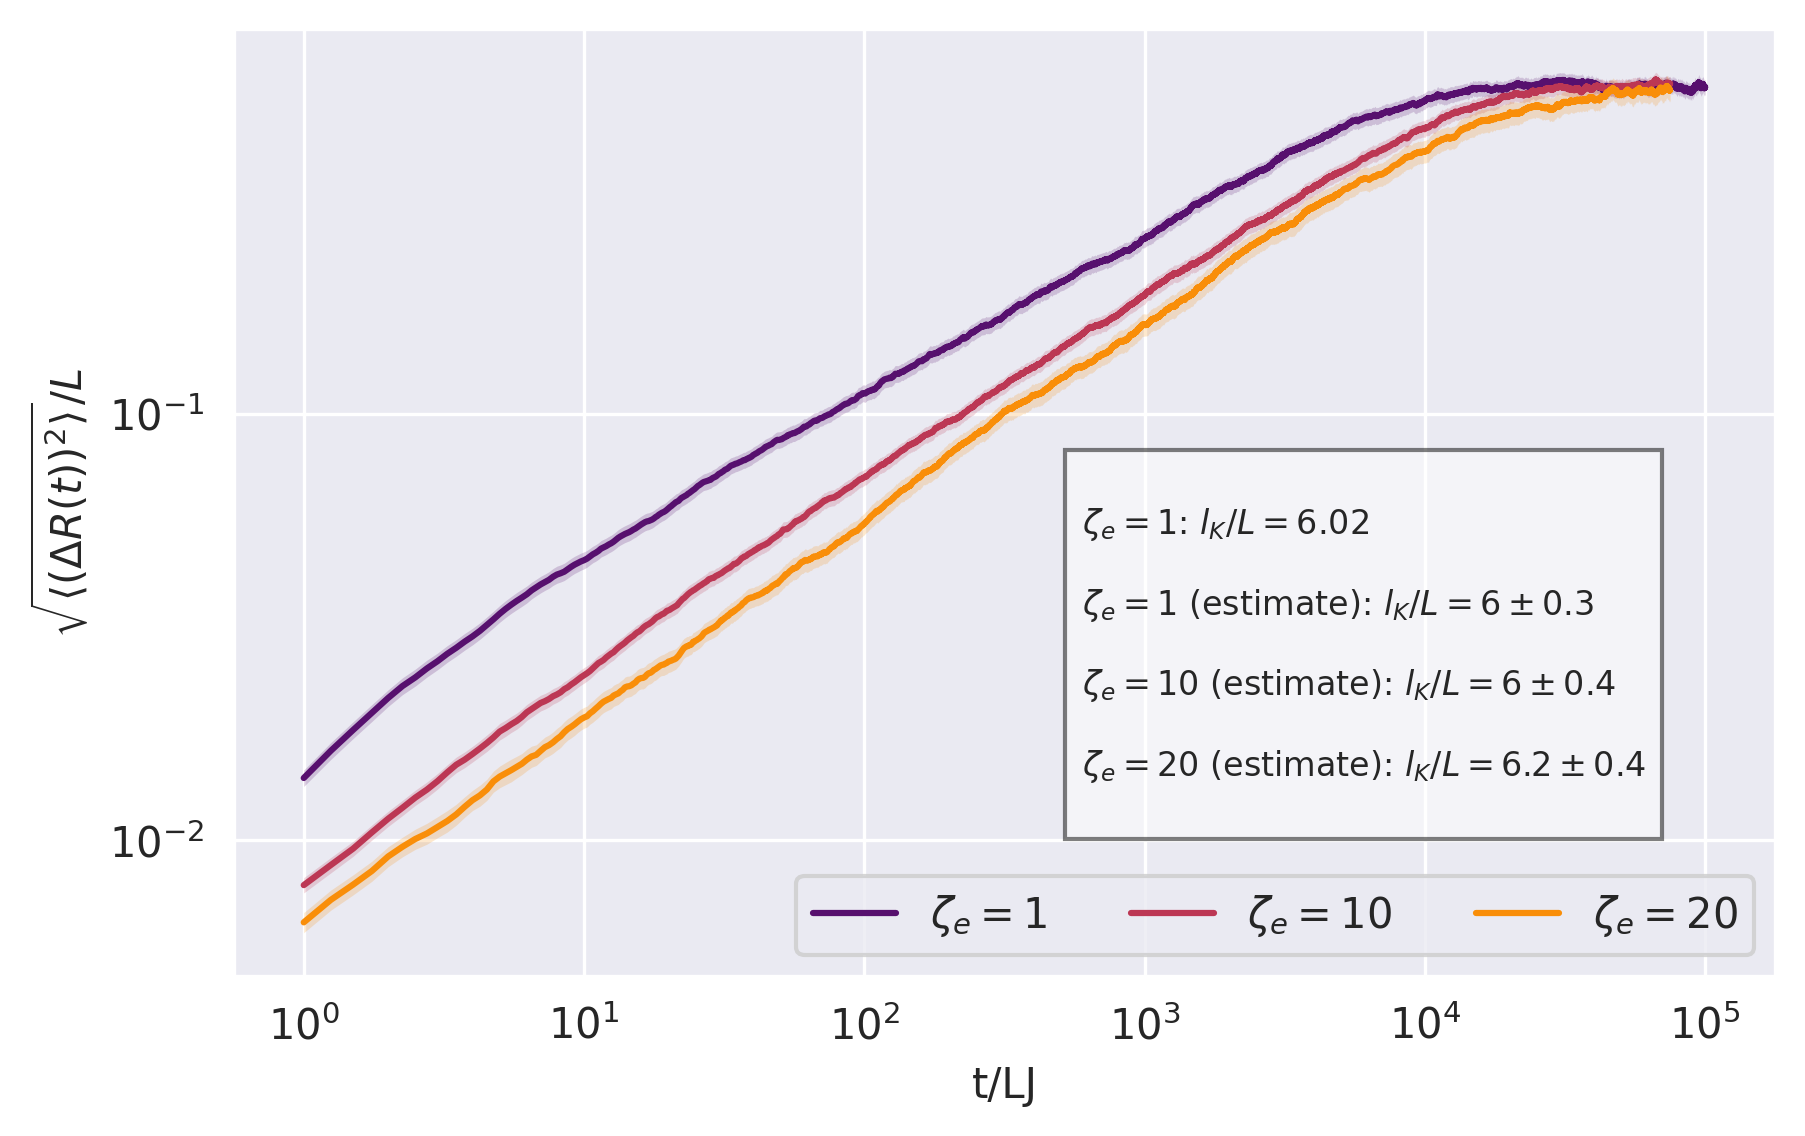
\includegraphics[width=10cm]{./14+15+16-exp-msd-log.png}
        \caption{Empirical MSD of ETE of anchored chains with different values of the friction
        coefficient of the chain end $\zeta_e$. Configured and estimated Kuhn length is shown in the text
        box (as additional check of plausibility).}
    \end{figure}
\end{frame}

% Semiflexible anchored impact of zeta_e - compare params ----------------------------------------

\begin{frame}
    \frametitle{Anchored semiflexible chains - impact of $\zeta_e$}
    \framesubtitle{MSD, compare parameters}
    \begin{figure}[h]
        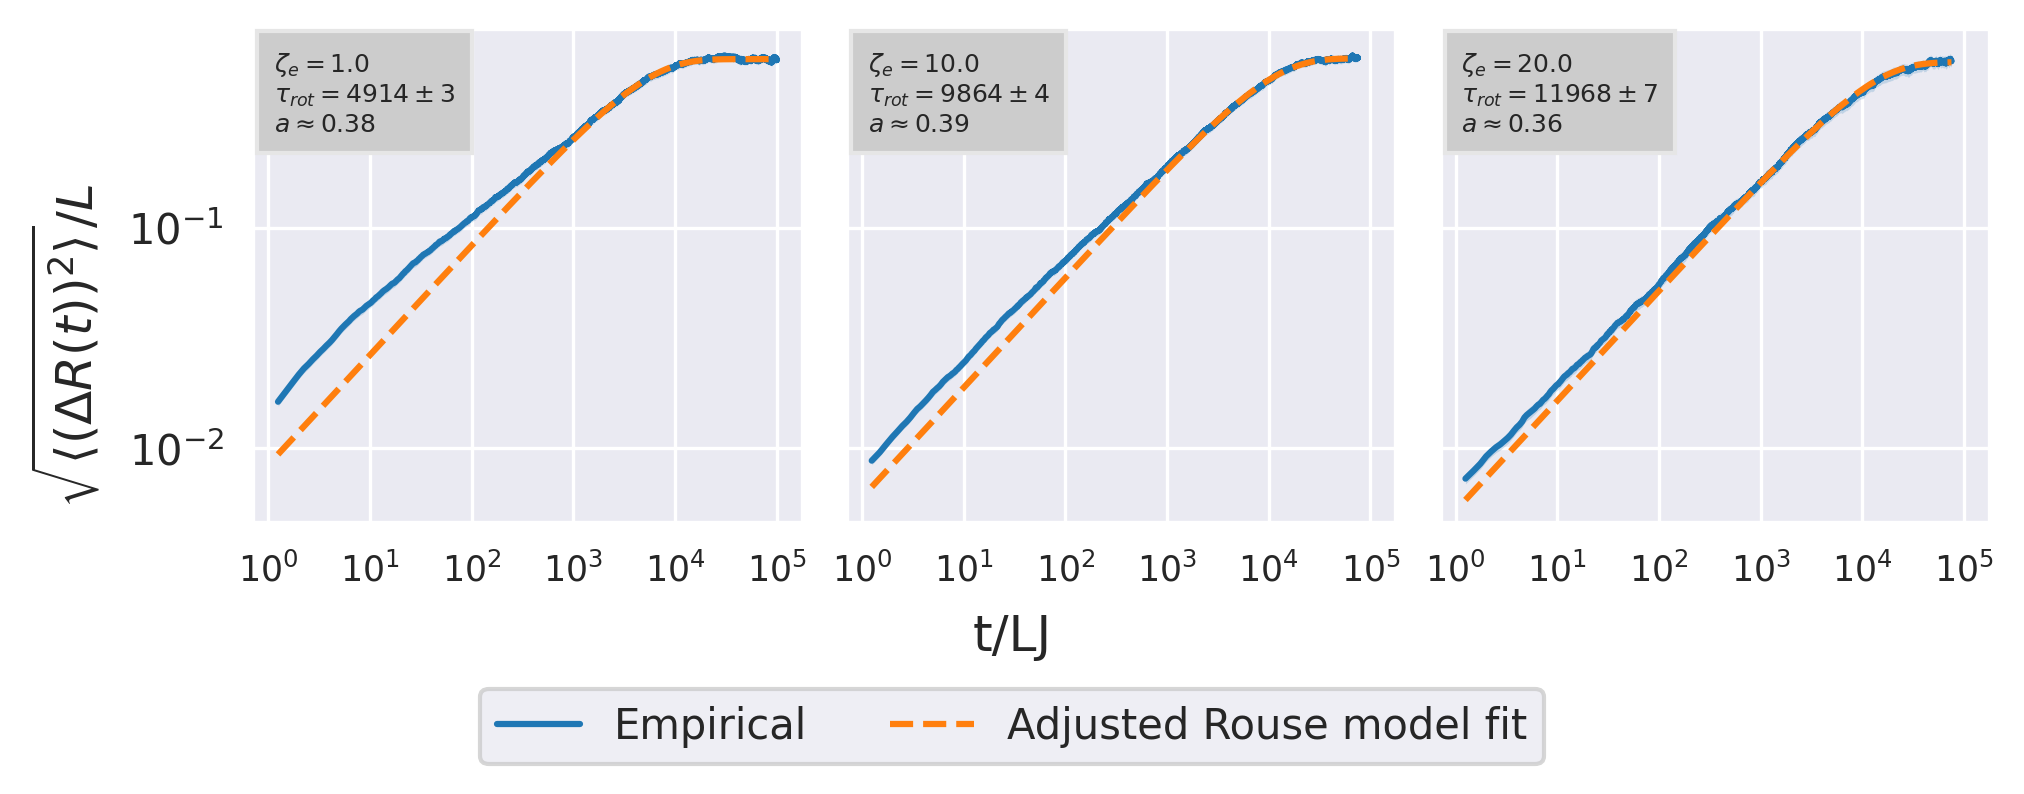
\includegraphics[width=\textwidth]{14+15+16-exp-msd-log-arm_fit-log.png}
        \caption{Empirical MSD of ETE of anchored chains with different values of
        the friction coefficient of the chain end $\zeta_e$ and a corresponding fit
        of the Adjusted Rouse model.
        }
    \end{figure}
\end{frame}

% Semiflexible anchored impact of zeta_e - alpha ----------------------------------------

\begin{frame}
    \frametitle{Anchored semiflexible chains - impact of $\zeta_e$}
    \framesubtitle{Scaling behavior}
    \begin{figure}[h]
        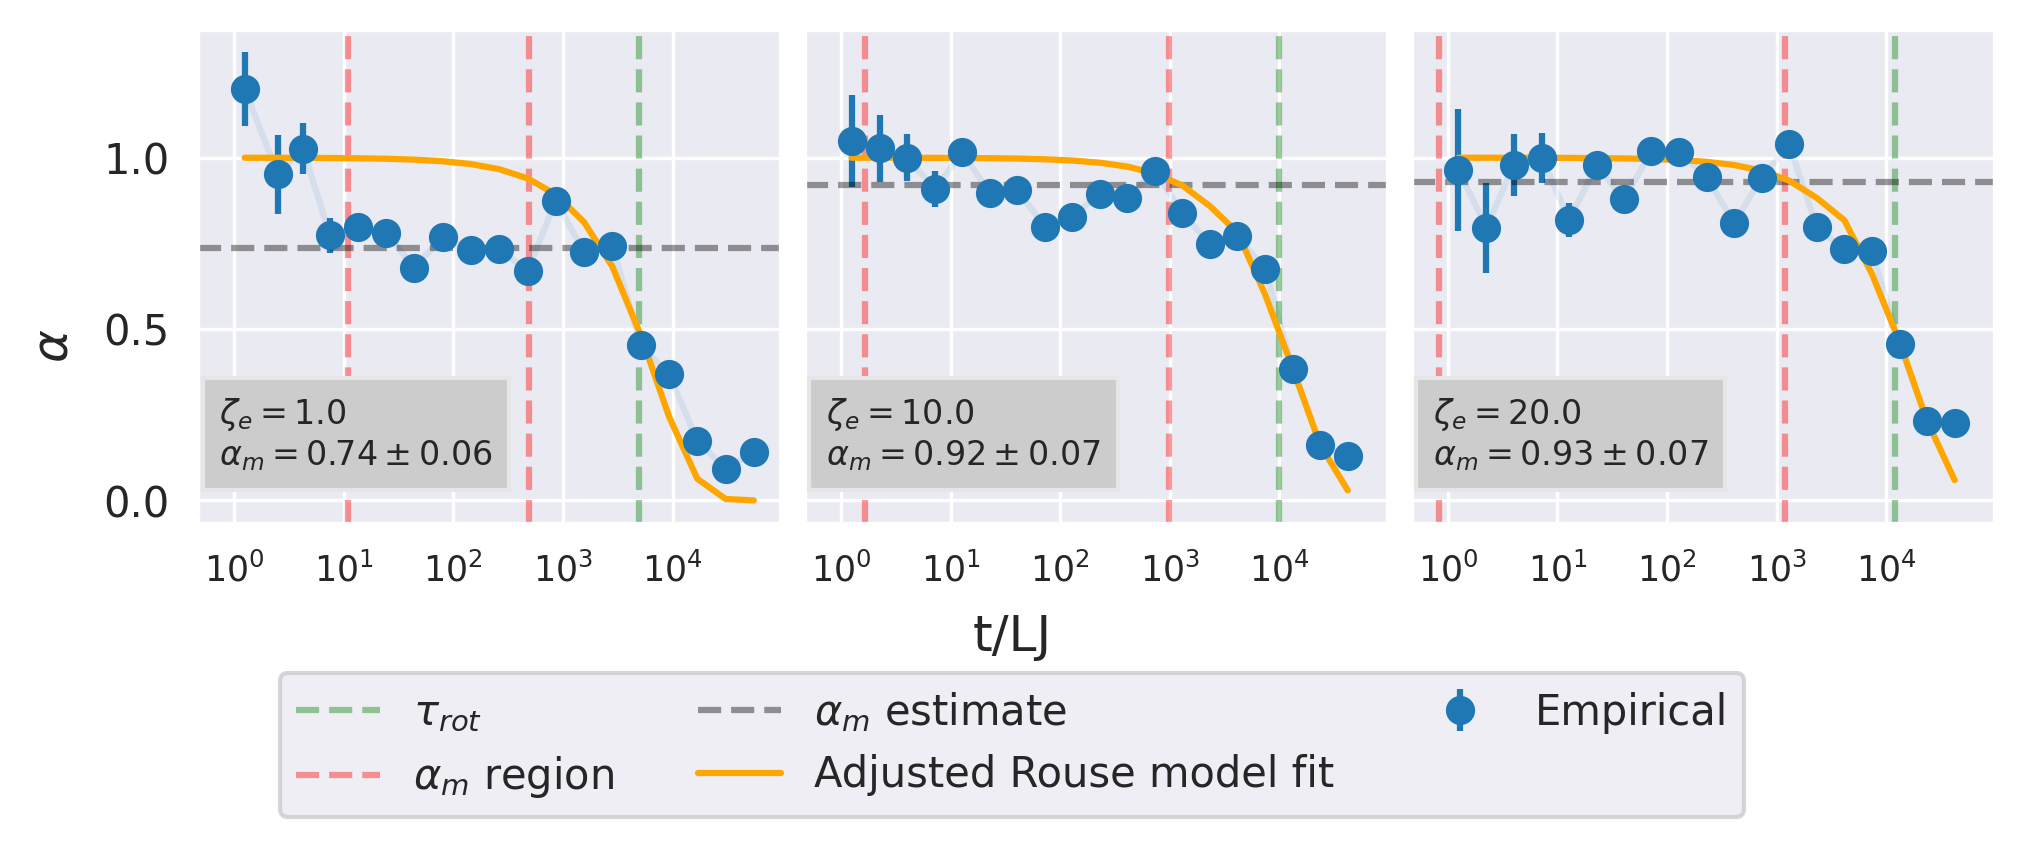
\includegraphics[width=\textwidth]{14+15+16-exp-alpha.png}
        \caption{Scaling exponent $\alpha$ of MSD of ETE 
        of anchored chains with different values of
        friction coefficient of the chain end $\zeta_e$ (blue dots).
        Estimated scaling exponent for the time interval
        $t \ll \tau_{rot}$: $\alpha_m$ (grey dashed line); Red dashed lines
        correspond to $\alpha_m$ scaling region which is estimated as:
        $[10 \frac{m_e}{\zeta_e}, \frac{\tau_{rot}}{10}]$
        }
    \end{figure}
\end{frame}

% Semiflexible anchored impact of zeta_e - conclusions ----------------------------------------

\begin{frame}
    \frametitle{Anchored semiflexible chains - impact of $\zeta_e$}
    \framesubtitle{Conclusions / Results}
    \begin{itemize}
        \item $l_K$ of the EEA1-like- and EEA1+Rab5-like- anchored chain is the same.
        \item Increased diameter of end monomer changes short- and interim-time scale 
        dynamics. Relaxation time of the chain increases. Likely because of slower
        diffusion of the end monomer and correspondingly of the part of the chain.
    \end{itemize}
\end{frame}


\section{Free chain dynamics}

% Free, smaller end - MSD ----------------------------------------

\begin{frame}
    \frametitle{Free chains}
    \framesubtitle{MSDLM, smaller chain end}
    \begin{figure}[h]
        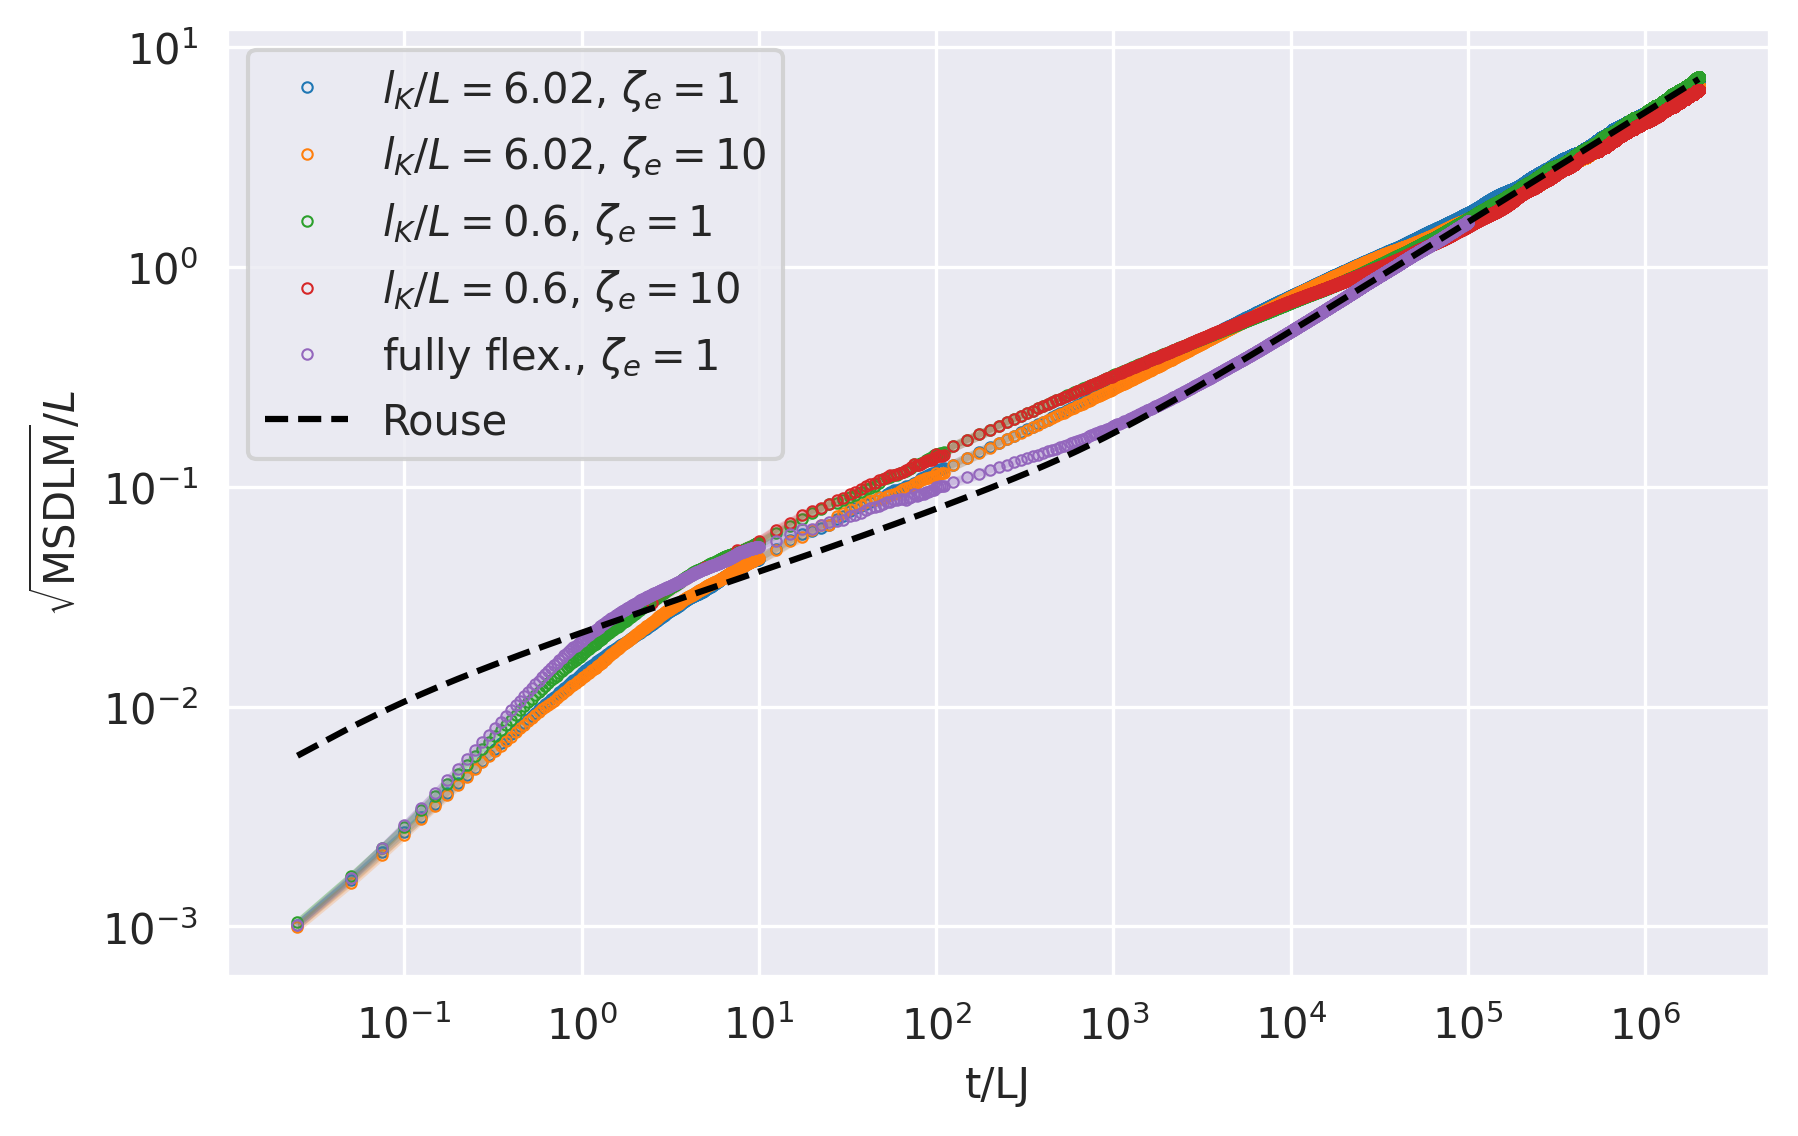
\includegraphics[width=0.9\textwidth]{17+18+19+20-exp-msd-fm-log.png}
        \caption{
            Empirical MSD of chain end (MSDLM) of free chains
            with different stiffness and end-bead friction values and
            Rouse model prediction for fully flexible chains.
        }
    \end{figure}
\end{frame}

% Free, smaller end - alpha ----------------------------------------

\begin{frame}
    \frametitle{Free chains}
    \framesubtitle{Scaling behavior, smaller chain end}
    \begin{figure}
        \centering
        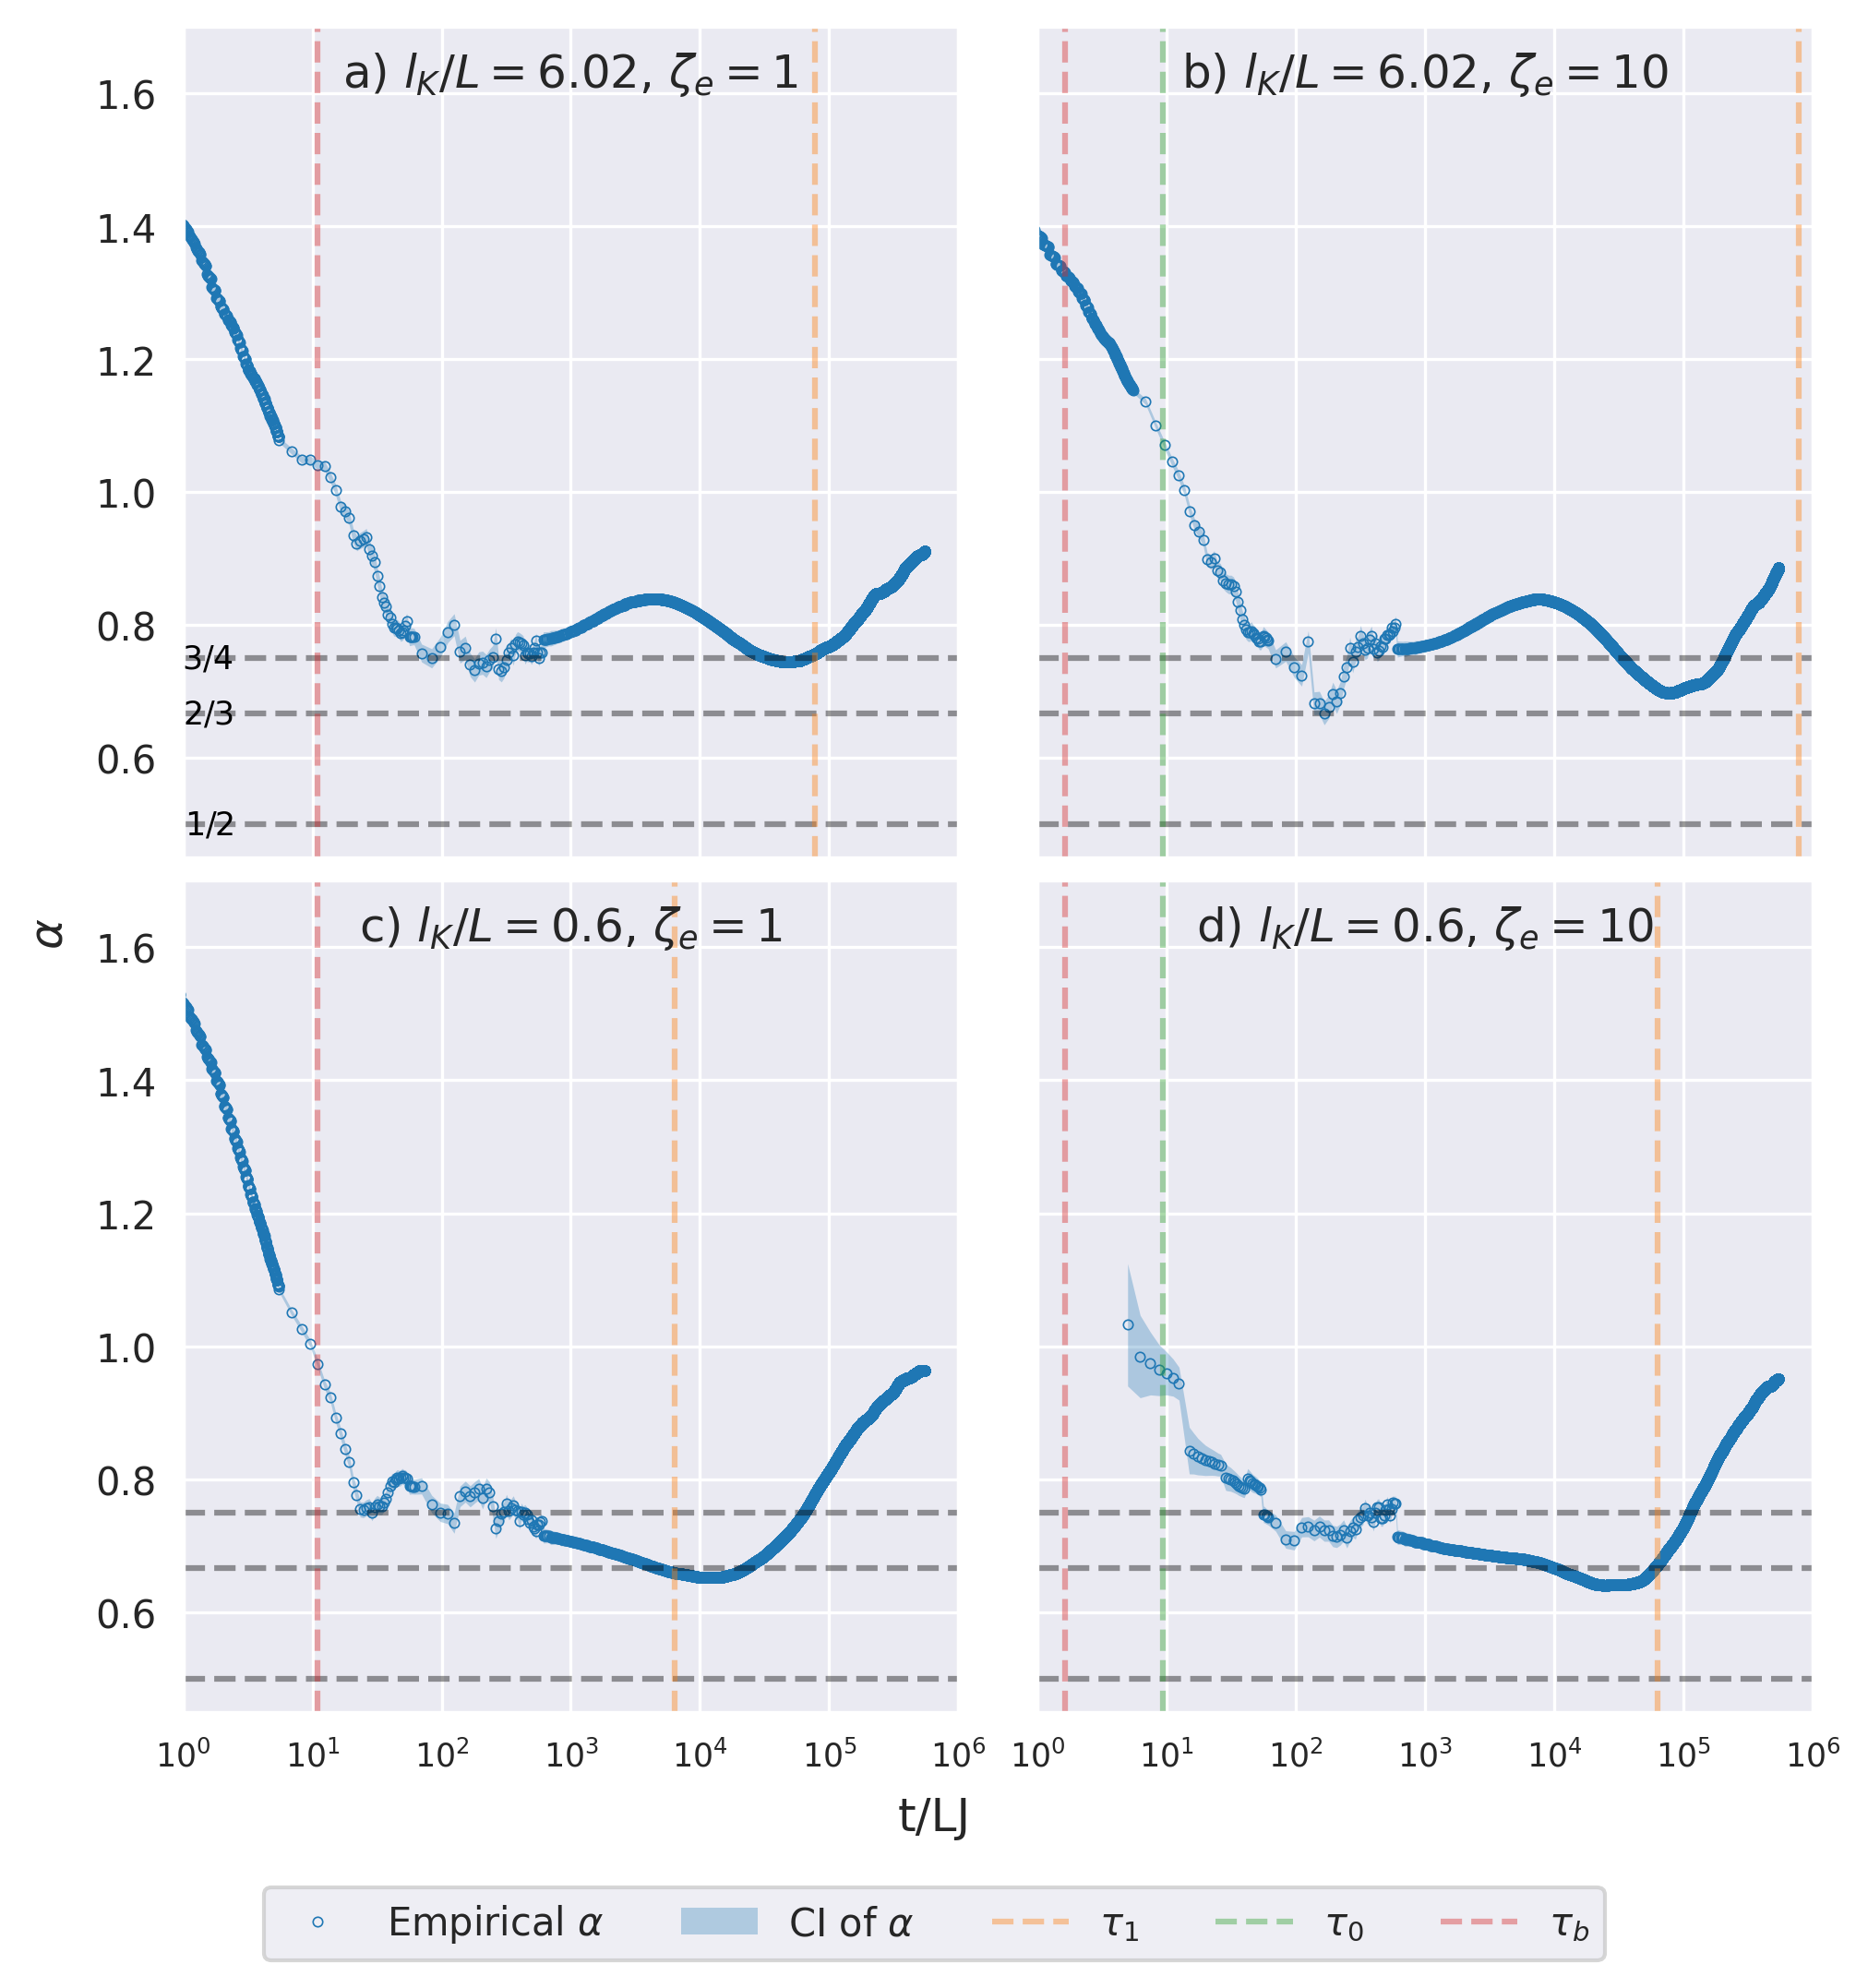
\includegraphics[width=0.6\textwidth]{17+18+19+20-exp-alpha-fm.png}
        \caption{Scaling exponent $\alpha$ of MSD of chain end (MSDLM) 
        of free chains with different stiffness and end-bead friction values
        }
        \label{fig:alpha_fm_free}
    \end{figure}
\end{frame}

\begin{frame}
    \frametitle{Free chains}
    \framesubtitle{Scaling behavior, smaller chain end}
    \begin{figure}
        \centering
        \begin{subfigure}{0.58\textwidth}
            \centering
            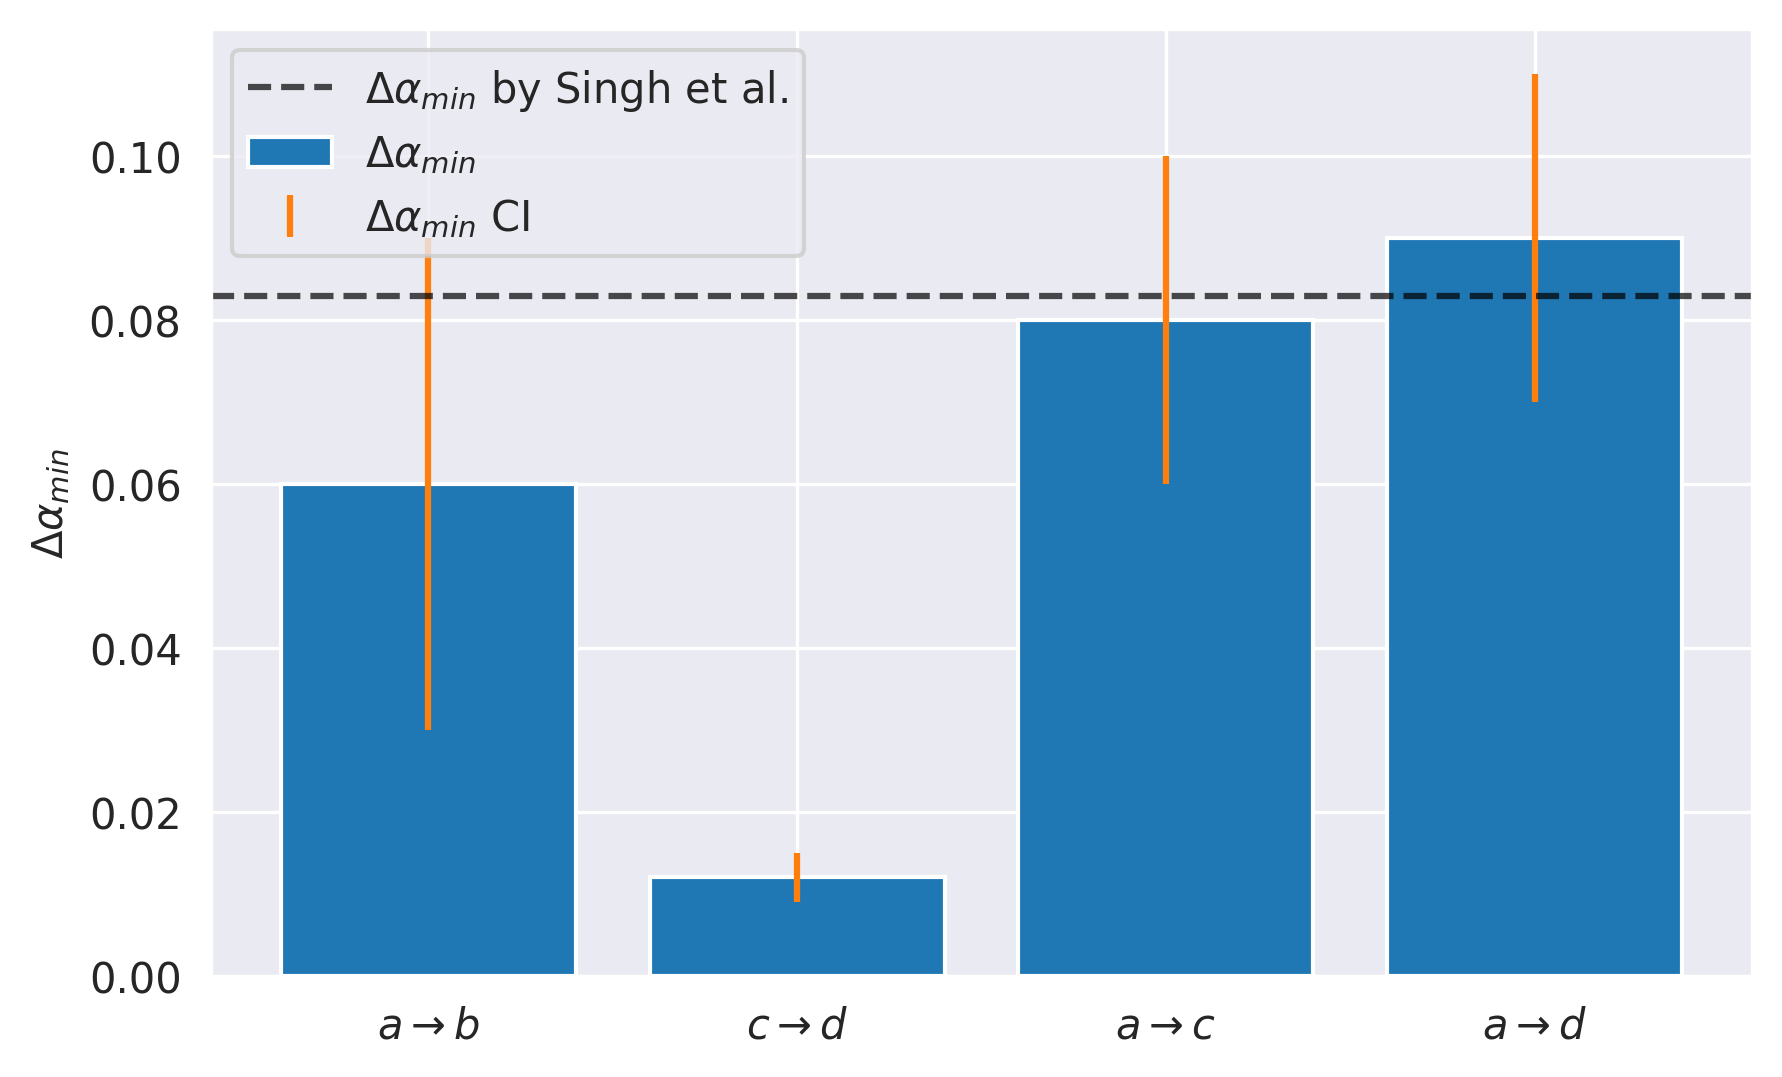
\includegraphics[width=\textwidth]{17+18+19+20-exp-delta_alpha_min_fm.png}
        \end{subfigure}
        \begin{subfigure}{0.4\textwidth}
            \centering
            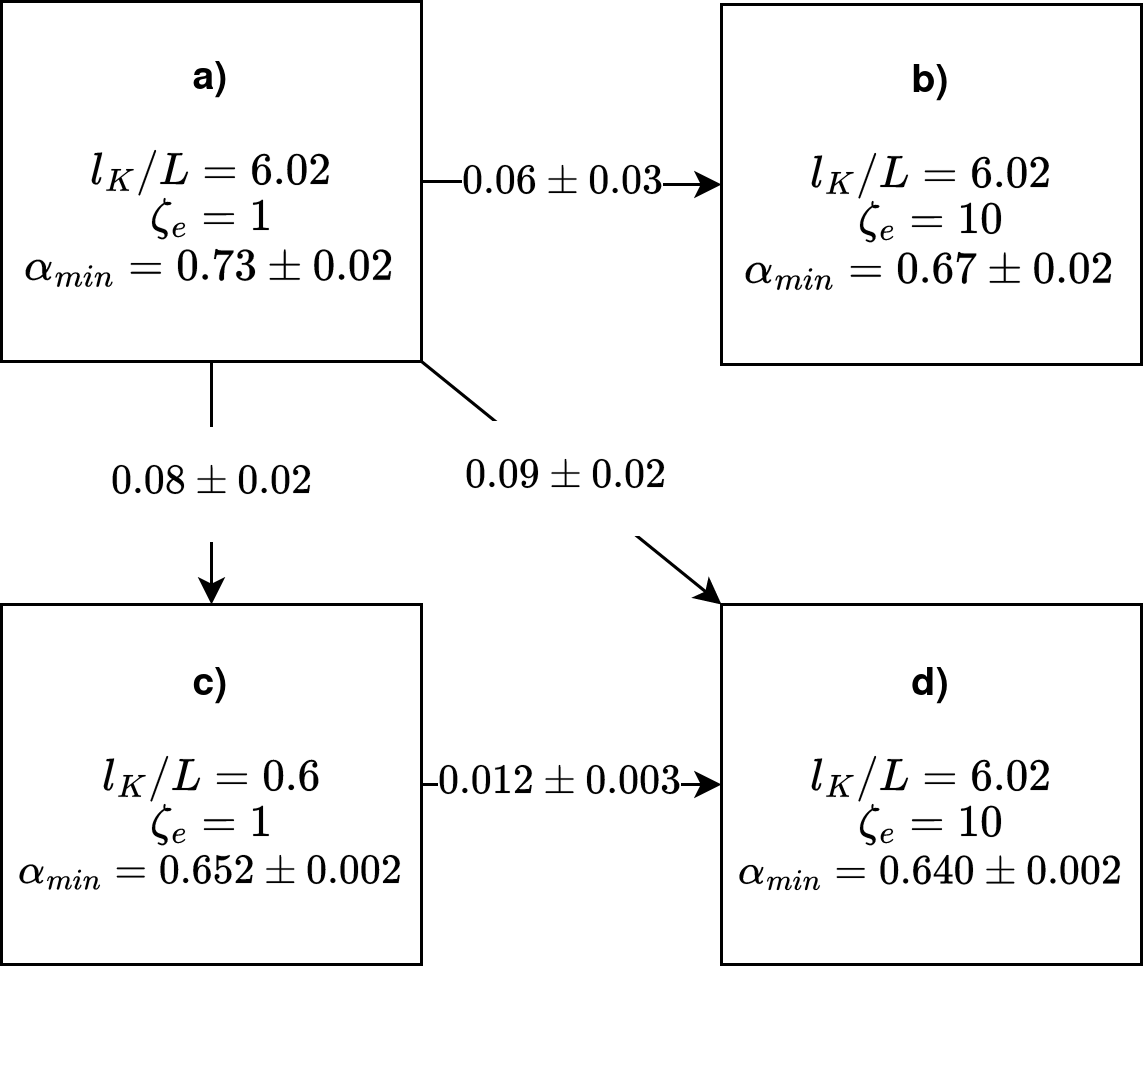
\includegraphics[width=\textwidth]{cases_diag.png}
        \end{subfigure}
    \end{figure}
\end{frame}

\begin{frame}
    \frametitle{Free chains}
    \framesubtitle{Conclusions}

\end{frame}

\begin{frame}
    \frametitle{Definitions, notations, units}
    Mostly: following \cite{svaneborg_2020}

    Units: LJ

    Notations and definitions:

    \begin{itemize}
        \item Contour length: $L$
        \item End to End distance (ETE): $\vec{R}$
        \item Change of ETE: $[\Delta R(t)]^2 := [\vec{R}(t)-\vec{R}(0)]^2$
        \item Friction coefficient of bead, viscosity: $\zeta$ $[\frac{\textrm{mass}}{\textrm{time}}]$, $\eta$ $[\frac{\textrm{mass}}{\textrm{time} * \textrm{distance}}]$
        \item subscript "$b$" to denote bead specific properties to distinguish these from Kuhn units:
            \begin{itemize}
                \item Kuhn lenght, bond length: $l_K$, $l_b$
                \item Number of Kuhn segments, number of beads: $N_K$, $N_b$
            \end{itemize}
        \item Friction coefficient of center of mass: $\zeta_{CM}=N_b \zeta$ 
        \item Rouse relaxation time \cite{svaneborg_2020}: $\tau_R = \frac{1}{3 \pi^2} \frac{\zeta_{CM} \mean{R^2}}{k_B T} = \frac{1}{3 \pi^2} \frac{\zeta N_b^2 l_b^2}{k_B T}$
        \item Relaxation time of single bead: $\tau_0 = \frac{3\pi^2 \tau_R}{N^2}$ 
    \end{itemize}

\end{frame}

\begin{frame}
    \frametitle{Definitions, notations, units}

    Notations and definitions:

    \begin{itemize}
        \item index "e" for variables referring end-monomer of the chain: $m_e$, $\zeta_e$ 
    \end{itemize}
    \vspace{1cm}
    Conventions:
    \begin{itemize}
        \item Confidence interval specification: $\pm 3\sigma$ (Normal distribution assumed)
    \end{itemize}
\end{frame}
    
\begin{frame}
    \frametitle{Common simulation settings and values}

    \begin{itemize}
        \item Only bonded beads interract (ideal chain)
        \item Chain parameters: 64 monomers, monomer mass $m=1$
        \item Ensemble size $ \ge $ 500 chains
        \item Environment parameters: $\zeta=1$
        \item Time step 0.0025 LJ
    \end{itemize}

\end{frame}

\section{References}

\setbeamertemplate{bibliography item}{\insertbiblabel}
\begin{frame}
    \frametitle{References}
    \bibliographystyle{apalike}
    \bibliography{sources}
\end{frame}

\section{Appendix}

\begin{frame}
    \frametitle{Experiment 2: Semi-flexible chain, vary persistence length}
    \framesubtitle{$\mean{[\Delta R(t)]^2}$ vs Rouse with $\tau_R$ analytically}

    \begin{figure}[h]
        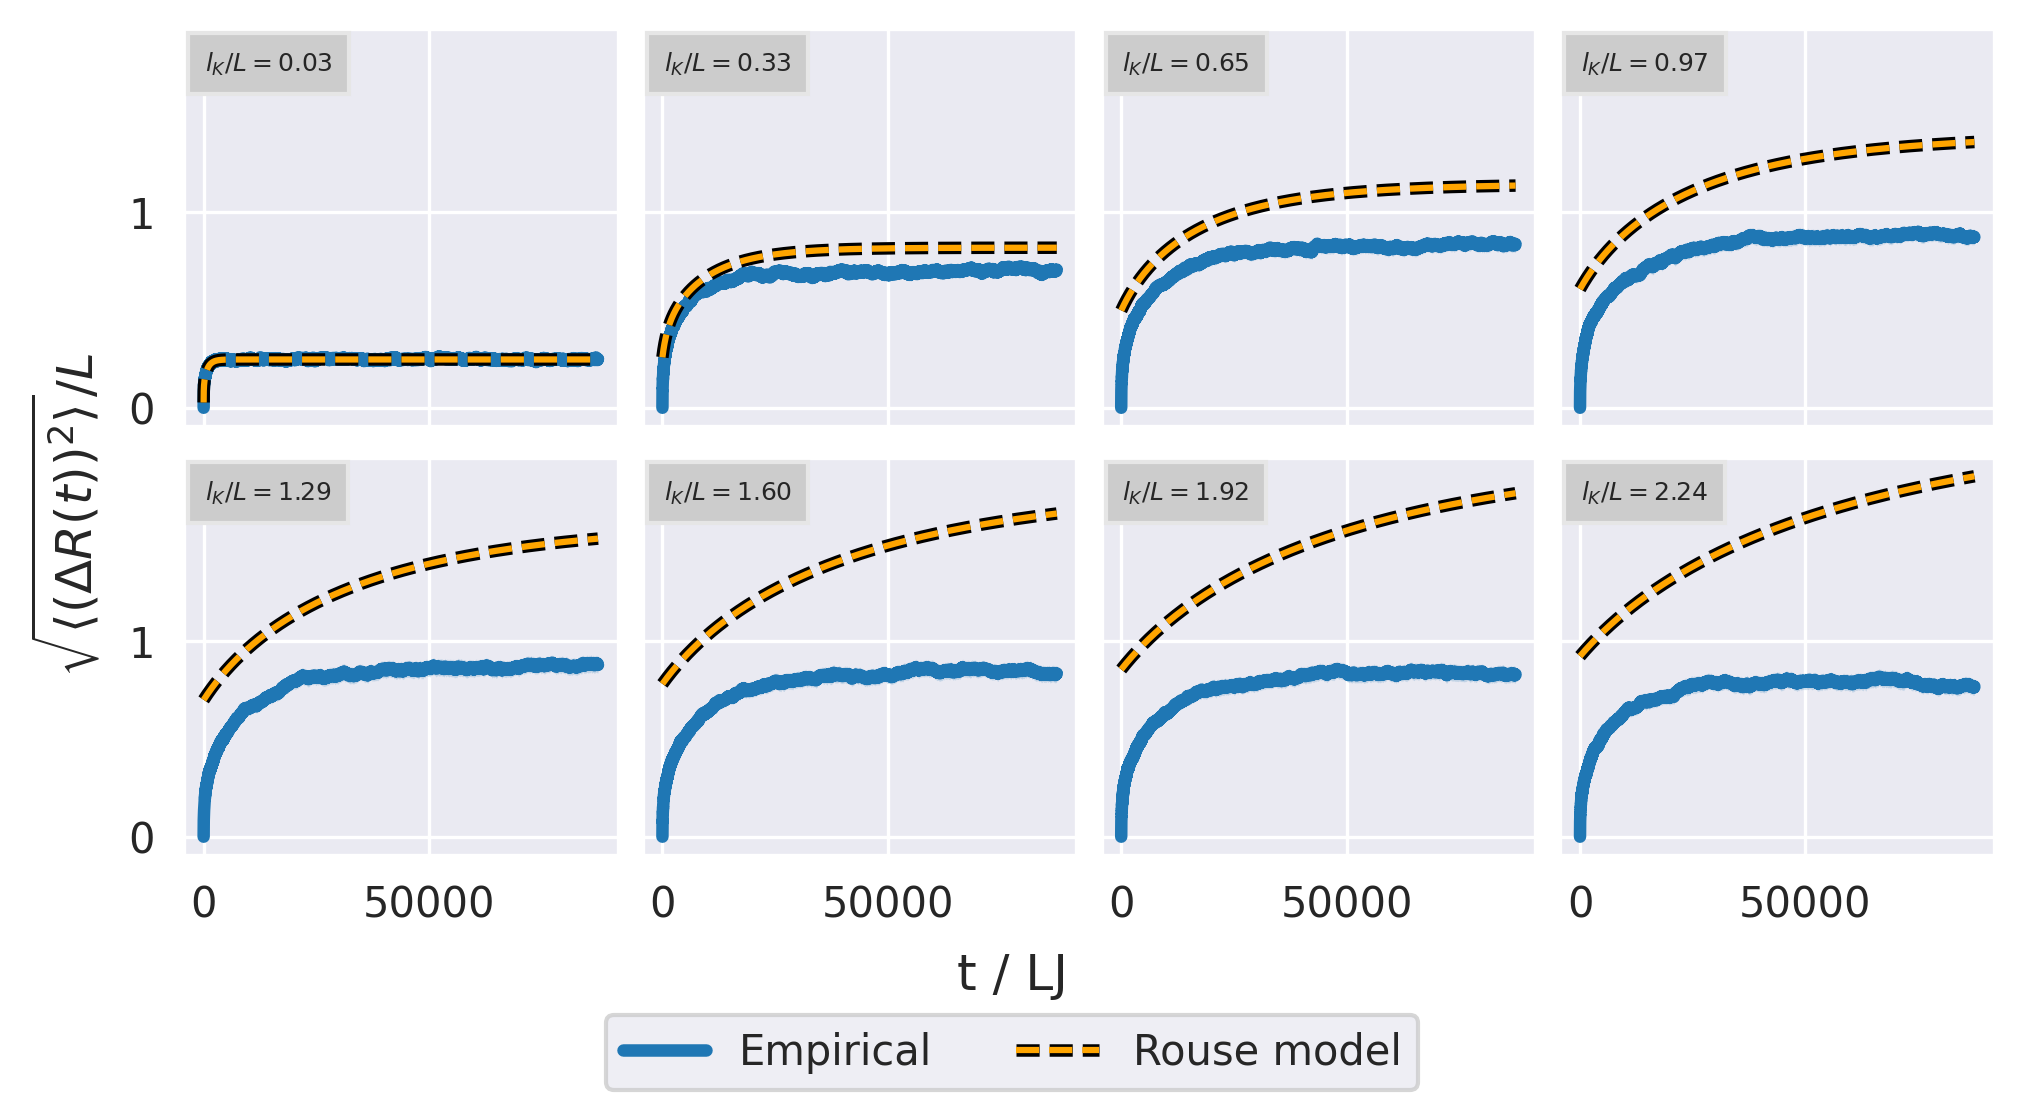
\includegraphics[width=11cm]{./4-exp-delta_R-rouse_anal.png}
    \end{figure}
\end{frame}

\begin{frame}
    \frametitle{Experiment 2: Semi-flexible chain, vary persistence length}
    \framesubtitle{$\mean{[\Delta R(t)]^2}$ vs Rouse with $\tau_R$ as free parameter}

    \begin{figure}[h]
        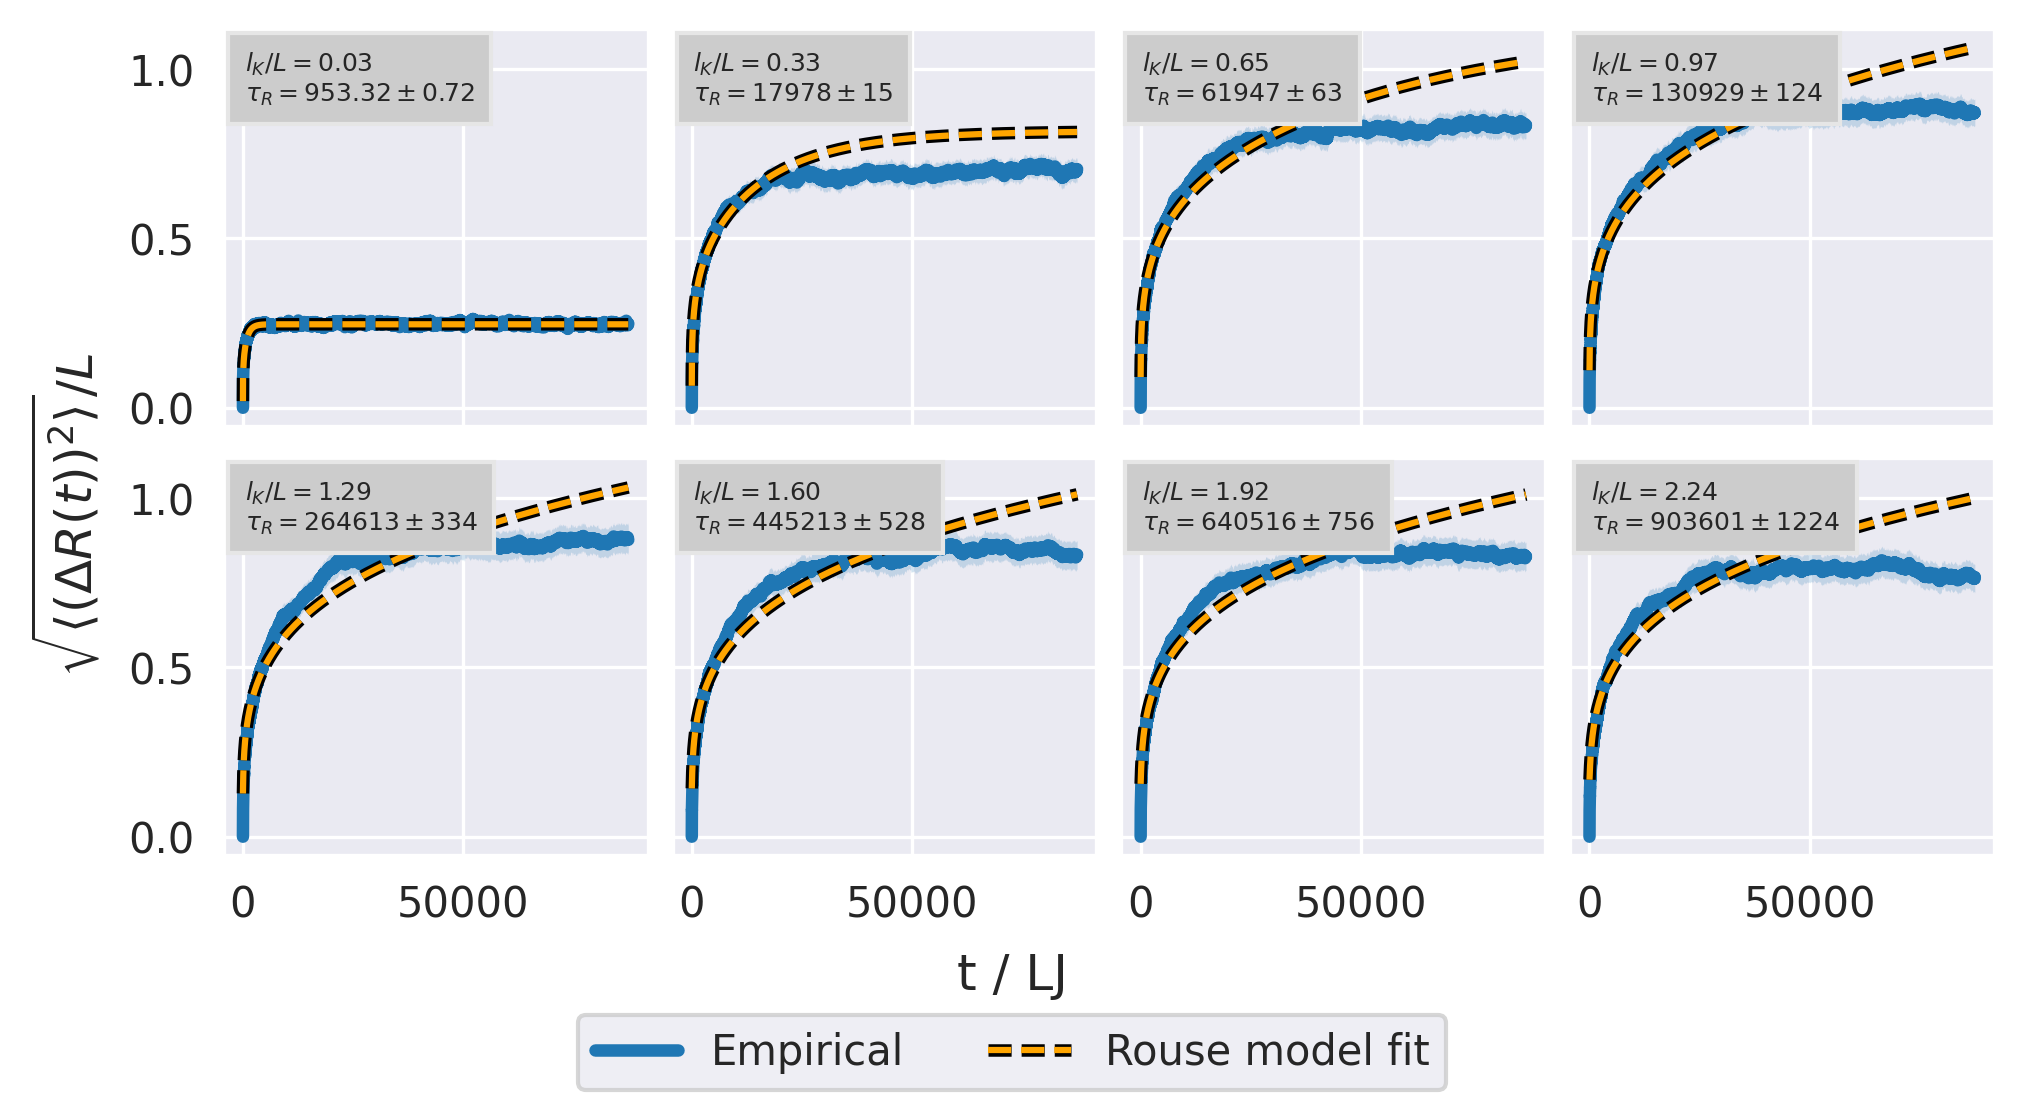
\includegraphics[width=11cm]{./4-exp-delta_R-rouse_fit-tau.png}
    \end{figure}
\end{frame}

\begin{frame}
    \frametitle{Experiment 2: Semi-flexible chain, vary persistence length}
    \framesubtitle{MSD: $\mean{[\Delta R(t)]^2}$ by dimension on log scale}

    \begin{figure}[h]
        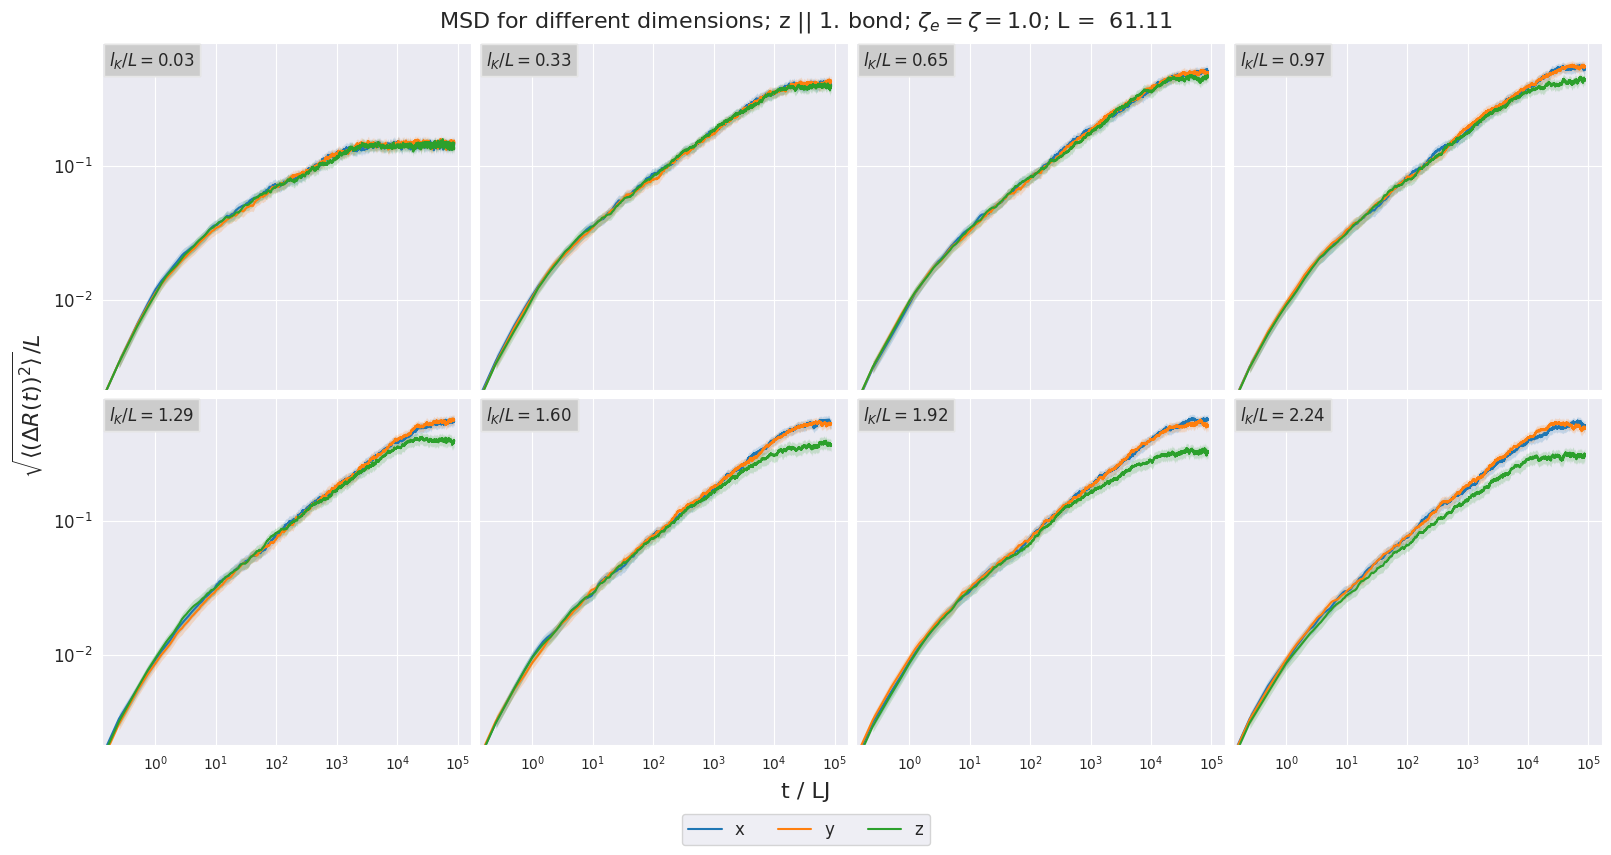
\includegraphics[width=11cm]{./4-exp-msd_by_dim-log.png}
    \end{figure}
\end{frame}

% Semiflexible anchored impact of zeta_e - by dim ----------------------------------------

\begin{frame}
    \frametitle{Anchored semiflexible chains - impact of $\zeta_e$}
    \framesubtitle{Separation of the dynamics into components parallel and perpendicular to the main-axis}
    \begin{figure}[h]
        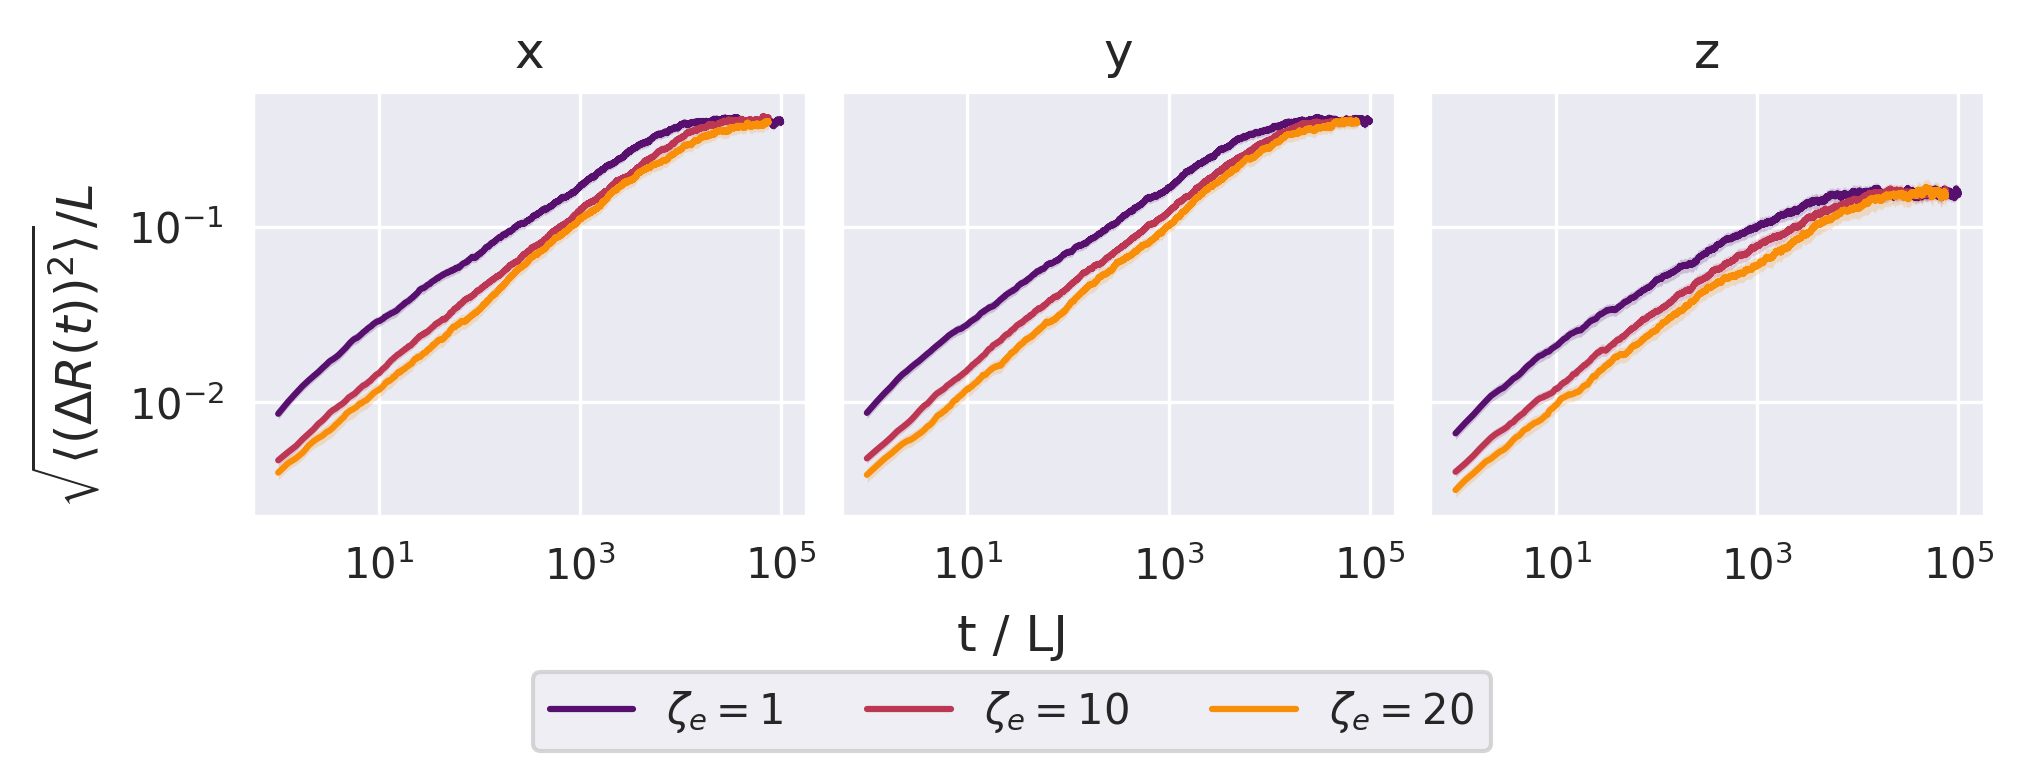
\includegraphics[width=11.2cm]{./14+15+16-exp-msd-dim-log.png}
        \caption{
        Empirical MSD of ETE of anchored chains with different values of the friction
        coefficient of the chain end $\zeta_e$, separated in components parallel and 
        perpendicular to the main-axis.
        }
    \end{figure}
\end{frame}

\end{document}